\documentclass[a4paper,12pt,oneside]{book} % nie: report!


% pakiety
\usepackage{polski} % lepiej to zamiast babel!
\usepackage[utf8]{inputenc} % w razie kłopotów spróbować: \usepackage[utf8x]{inputenc}
\usepackage{fancyhdr} % nagłówki i stopki
\usepackage{indentfirst} % WAŻNE, MA BYĆ!
\usepackage{lipsum}
\usepackage[pdftex]{graphicx} % to do wstawiania rysunków
\usepackage{amsmath} % to do dodatkowych symboli, przydatne
\usepackage[pdftex,
            left=1in,right=1in,
            top=1in,bottom=1in]{geometry} % marginsy
\usepackage{amssymb} % to też do dodatkowych symboli, też przydatne
\usepackage{pdfpages} % żeby wstawić stronę tytułową
% jesli potrzeb, można oczywiście wstawić inne pakiety i swoje definicje...
\usepackage{graphicx}
\graphicspath{{./pictures}}
\usepackage{caption}
\DeclareCaptionType{code}[Listing][Spis Listingów]

\usepackage{pgfplots}
\usepackage[backend=bibtex, sorting=none]{biblatex}
\addbibresource{./cytowania/cytowania.bib}

\usepackage{xstring}
\usepackage{tikz}
\usepackage{listofitems}
\usepackage{etoolbox}
\usepackage{listings}
\usetikzlibrary{arrows.meta, fit, positioning} % for arrow size
\usepackage[outline]{contour} % glow around text
\contourlength{1.4pt}
\tikzstyle{mynode}=[thick,draw=blue,fill=blue!20]
\usetikzlibrary{shapes, positioning}
\tikzset{>=latex} % for LaTeX arrow head
\usepackage{xcolor}
\colorlet{myred}{red!80!black}
\colorlet{myblue}{blue!80!black}
\colorlet{mygreen}{green!60!black}
\colorlet{myorange}{orange!70!red!60!black}
\colorlet{mydarkred}{red!30!black}
\colorlet{mydarkblue}{blue!40!black}
\colorlet{mydarkgreen}{green!30!black}
\tikzstyle{node}=[thick,circle,draw=myblue,minimum size=22,inner sep=0.5,outer sep=0.6]
\tikzstyle{node in}=[node,green!20!black,draw=mygreen!30!black,fill=mygreen!25]
\tikzstyle{node hidden}=[node,blue!20!black,draw=myblue!30!black,fill=myblue!20]
\tikzstyle{node out}=[node,red!20!black,draw=myred!30!black,fill=myred!20]
\tikzstyle{connect}=[thick,mydarkblue] %,line cap=round
\tikzstyle{connect arrow}=[-{Latex[length=4,width=3.5]},thick,mydarkblue,shorten <=0.5,shorten >=1]
\tikzset{ % node styles, numbered for easy mapping with \nstyle
	node 1/.style={node in},
	node 2/.style={node hidden},
	node 3/.style={node out},
}
\def\nstyle{int(\lay<\Nnodlen?min(2,\lay):3)} % map layer number onto 1, 2, or 3

% VAE
\newcommand\drawEncoder[2]{
	% #1 (str): namespace
	% #2 (list[list[str]]): list of labels to print in the node of each neuron
	\foreach \neurons [count=\lyrIdx] in #2 {
		\ifnum \lyrIdx = 1
			\StrCount{\neurons}{,}[\lyrLength]
			\foreach \n [count=\nIdx] in \neurons
			\node[myin] (#1-\lyrIdx-\nIdx) at (2*\lyrIdx, \lyrLength/2-1.4*\nIdx) {$x_\nIdx$};
		\else 
			\StrCount{\neurons}{,}[\lyrLength] 
			\foreach \n [count=\nIdx] in \neurons
			\node[hidden] (#1-\lyrIdx-\nIdx) at (2*\lyrIdx, \lyrLength/2-1.4*\nIdx) {\n};
		\fi
	}
}

\newcommand\drawDecoder[2]{
	% #1 (str): namespace
	% #2 (list[list[str]]): list of labels to print in the node of each neuron
	\foreach \neurons [count=\lyrIdx] in #2 {
		\ifnum \lyrIdx = 3
			\StrCount{\neurons}{,}[\lyrLength]
			\foreach \n [count=\nIdx] in \neurons
			\node[myout] (#1-\lyrIdx-\nIdx) at (2*\lyrIdx, \lyrLength/2-1.4*\nIdx) {$\hat{x}_\nIdx$};
		\else 
			\StrCount{\neurons}{,}[\lyrLength] 
			\foreach \n [count=\nIdx] in \neurons
			\node[hidden] (#1-\lyrIdx-\nIdx) at (2*\lyrIdx, \lyrLength/2-1.4*\nIdx) {\n};
		\fi
	}
}
\newcommand\denselyConnectNodes[2]{
	% #1 (str): namespace
	% #2 (list[int]): number of nodes in each layer
	\foreach \n [count=\lyrIdx, remember=\lyrIdx as \previdx, remember=\n as \prevn] in #2 {
		\foreach \y in {1,...,\n} {
			\ifnum \lyrIdx > 1
			\foreach \x in {1,...,\prevn}
			\draw[connect] (#1-\previdx-\x) -- (#1-\lyrIdx-\y);
			\fi
		}
	}
}


% definicje nagłówków i stopek
\pagestyle{fancy}
\renewcommand{\chaptermark}[1]{\markboth{#1}{}}
\renewcommand{\sectionmark}[1]{\markright{\thesection\ #1}}
\fancyhf{}
\fancyhead[LE,RO]{\footnotesize\bfseries\thepage}
\fancyhead[LO]{\footnotesize\rightmark}
\fancyhead[RE]{\footnotesize\leftmark}
\renewcommand{\headrulewidth}{0.5pt}
\renewcommand{\footrulewidth}{0pt}
\addtolength{\headheight}{1.5pt}
\fancypagestyle{plain}{\fancyhead{}\cfoot{\footnotesize\bfseries\thepage}\renewcommand{\headrulewidth}{0pt}}

% interlinia
\linespread{1.25}


% treść
\begin{document}
\sloppy

\thispagestyle{empty}

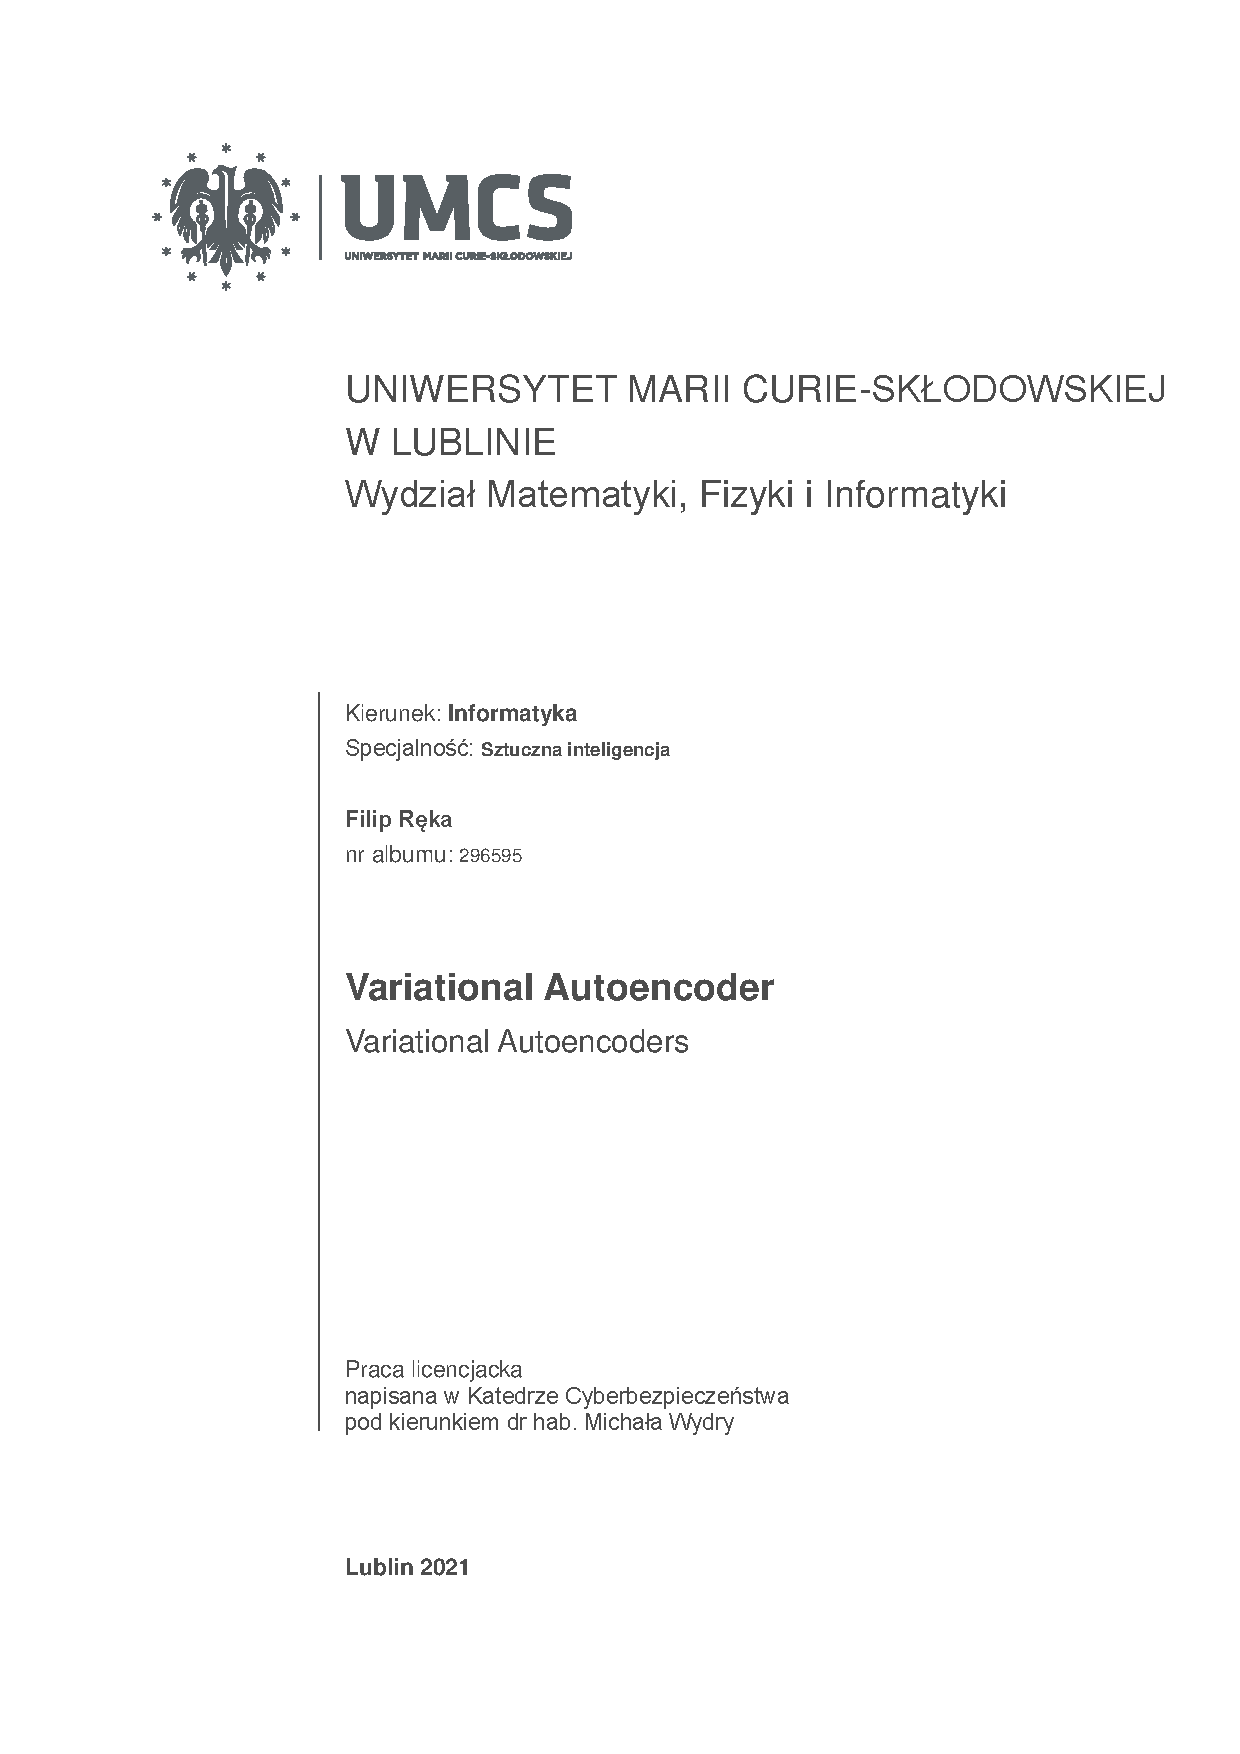
\includepdf{stronatytulowasvg}

\tableofcontents{}

\chapter*{Wstęp} % z gwiazdką, więc bez numerka...
\addcontentsline{toc}{chapter}{Wstęp} % ...ale w spisie treści ma być
\textbf{Autoenkoder} jest jednym z rodzajów sieci neuronowych, której zadaniem jest nauczenie się zakodowania nieoznaczonych danych. Kod jest wykorzystywany do ponownego i jak najlepszego, wygenerowania wejścia sieci. Autoenkoder uczy się reprezentacji zbioru danych jako zmiennych ukrytych przez ignorowanie nieistotnych części danych.
Wariacyjne autoenkodery są popularnymi modelami generacyjnymi. Zostały zaproponowane przez Diederika P. Kingma i Maxa Wellinga w roku 2014 \cite{kingma2014autoencoding}. Najczęściej zostają one skategoryzowane do modeli uczenia częściowo nadzorowanego. Znajdują zastosowanie w generacji obrazów, tekstu, muzyki oraz w detekcji anomalii. W przeciwieństwie do tradycyjnych autoenkoderów prezentują probabilistyczne podejście do generowania zmiennych ukrytych. Swoją popularność zawdzięcza swojej budowie, która jest oparta na sieciach neuronowych oraz możliwości trenowania ich przy pomocy metod gradientowych.
\chapter*{Cel i zakres pracy}
\addcontentsline{toc}{chapter}{Cel i zakres pracy}
Celem pracy jest przegląd i ocena możliwości dwóch popularnych modeli uczenia maszynowego: tradycyjnego oraz wariacyjnego autoenkodera. Oba modele, mimo podobieństwa w nazwie, różnią się budową oraz zastosowaniami. Jako modele kompresujące dane, są wykorzystywane do redukcji wymiarów, odszumiania danych oraz detekcji anomalii. Tradycyjna konstrukcja modelu, w przeciwieństwie do wariacyjnej, nie nadaje się do generacji danych, takich jak obrazów lub ścieżek audio \cite{vaeaudio}. W pracy zostanie wytłumaczony ten problem i na podstawie matematycznych formuł wyprowadzona będzie struktura generacyjnego modelu. Dla obu modeli przedstawiono ich typowe zastosowania oraz zostały zaimplementowane w języku Python w bibliotece TensorFlow.
\chapter{Tradycyjny autoenkoder}
\section{Informacje wstępne}
Autoenkoder (AE) jest specyficzną wersją sieci neuronowej składającej się z dwóch części: enkodera, który koduje dane wejściowe oraz dekodera, który na podstawie kodu rekonstruuje wejście \cite{bank2021autoencoders}. Architektura enkodera wymaga, aby jego warstwa wyjściowa generująca reprezentacje danych była mniejsza niż warstwa wejściowa. Często zwężenie to jest nazywane \textit{bottleneck}. Model na swoją warstwę wejściową oraz wyjściową dostaje te same dane. Posiadając dane wejściowe $X$ o wymiarze $m$ oraz chcąc je zakodować do wymiaru $n$, można formalnie zapisać:

\begin{center}
	Enkoder E: $\mathbb{R}^m \rightarrow \mathbb{R}^n$\\
	Dekoder D: $\mathbb{R}^n \rightarrow \mathbb{R}^m$\\
	gdzie $n < m$\\
\end{center}
Celem \textit{bottleneck-a} jest skompresowanie wejścia i zachowanie w ukrytych wartościach jak najwięcej informacji. W momencie, kiedy $n = m$, model przekazałby wartości z pierwszej warstwy na ostatnią bez potrzeby kompresji. Celem treningu całego autoenkodera jest zminimalizowanie błędu pomiędzy prawdziwymi danymi wejściowymi a tymi odkodowanymi ze skompresowanych wartości. W przypadku obrazów funkcją straty może być na przykład błąd średniokwadratowy \ref{equ:aeloss} lub entropia krzyżowa \ref{equ:entropy}, która powie, jak wynik różni się od wejścia. 
 \begin{equation}
 		 \mathcal{L}(x, \hat{x}) = \dfrac{1}{m}\displaystyle\sum_{i=0}^{m}(x_i-\hat{x}_i)^2 =\dfrac{1}{m}\displaystyle\sum_{i=0}^{m}(x_i-D(E(x_i)))^2
 		 \label{equ:aeloss}
 \end{equation}
 \begin{equation}
	\mathcal{L}(x, \hat{x}) = -\dfrac{1}{m}\displaystyle\sum_{i=0}^{m}(x_i\log(\hat{x}_i) + (1 -x_i)\log(1-\hat{x}_i))
	\label{equ:entropy}
\end{equation}
\begin{center}
	gdzie $x$ jest wejściem, $\hat{x}$ jego rekonstrukcją, a $m$ wymiarem danych
\end{center}
Kompresje obrazu do wektora kodu, a następnie jego rekonstrukcje przedstawiono na schemacie \ref{fig:aeschemat} \cite{bank2021autoencoders}.


\begin{figure}[h!]
	\centering
	\begin{tikzpicture}
		\node (true) at (-6, 0) {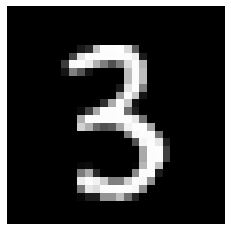
\includegraphics[width=3.5cm]{aeorg.png}};
		\draw[thick] (-3.4, 1.5) -- (-3.4, -1.5) node[pos=0.5] (enkoderin){} -- (-1.7, -0.8) -- (-1.7, 0.8) node[pos=0.5] (enkoderout){} -- cycle;
		\draw[-latex, thick] (true.east) -- (enkoderin.west);    
				\node[scale=0.7] (sample) at (0, 0) {\(\begin{bmatrix}
				3.18 \\ 1.83 \\ \vdots \\ 0.71 \\ 2.94
			\end{bmatrix}\)};                                     
		\draw[-latex, thick](enkoderout.east) -- (sample.west);                                                                                 
		\draw[thick] (1.7, 0.8) -- (1.7, -0.8) node[pos=0.5] (dekoderin){} -- (3.4, -1.7) -- (3.4, 1.7) node[pos=0.5] (dekoderout){} -- cycle;
		\node (recon) at (6, 0) {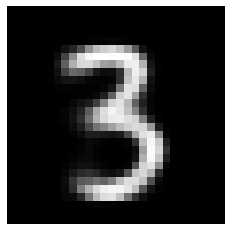
\includegraphics[width=3.5cm]{aerec.png}};
		\draw[-latex, thick](sample.east) -- (dekoderin.west);
		\draw[-latex, thick](dekoderout.east) -- (recon.west);
		% Labels
		\node at (-6, -2.2) {wejście};
		\node at (6, -2.2) {wyjście};
		\node at (0, -1.5) {wektor kodu};
		\node at (-2.52, 0) {enkoder};
		\node at (2.52, 0) {dekoder};
		
	\end{tikzpicture}
	\caption{Schemat budowy autoenkodera}
	\label{fig:aeschemat}
\end{figure}
\newpage
\subsection{Zbiór danych MNIST}
Zbiór danych Modified National Institute of Standards and Technology (MNIST) jest zbiorem wielu odręcznie pisanych cyfr \cite{mnist}. Znajduje szerokie zastosowanie w nauce i prezentacjach możliwości modeli uczenia maszynowego. W jego skład wchodzi 60 000 obrazów przeznaczonych do treningu modeli oraz 10 000 do testów. Obrazy są czarno-białe i mają wymiary 28 na 28 pikseli.
\begin{figure}[h]
	\centering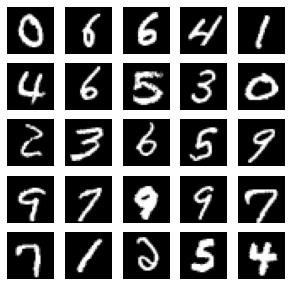
\includegraphics[width=7cm]{pictures/mnist.png}
	\caption{Przykładowe obrazy ze zbioru danych}
\end{figure}

W pracy zbiór ten jest wykorzystywany w celu pokazania różnic w budowie i zastosowaniu tradycyjnych oraz wariacyjnych autoenkoderów, dlatego że na obrazach łatwo zobaczyć zachowanie kompresji i rekonstrukcji. Cyfry są również bardzo łatwe do sklasyfikowania dla człowieka, przez co nowe wygenerowane dane są proste do porównania z tymi należącymi do zbioru danych.
\newpage
\section{Budowa autoenkoderów}
W skład autoenkodera wchodzi enkoder oraz dekoder. Obie części są w pełni połączonymi sieciami neuronowymi, połączonymi również pomiędzy sobą. Prosta budowa sprawia, że bez problemu obie sieci są trenowane równocześnie.
\begin{figure}[!h]
\centering
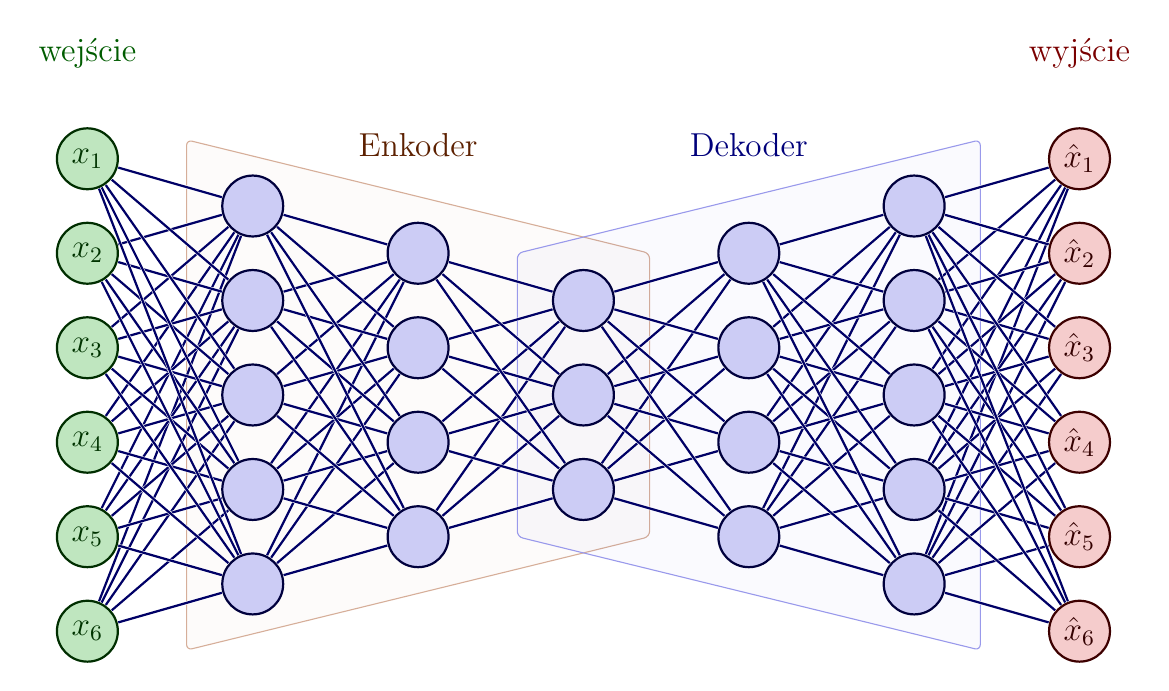
\begin{tikzpicture}[x=2.1cm,y=1.2cm]
	\large
	\readlist\Nnod{6,5,4,3,4,5,6} % array of number of nodes per layer
	
	% TRAPEZIA
	\node[above,align=center,myorange!60!black] at (3,2.4) {Enkoder};
	\node[above,align=center,myblue!60!black] at (5,2.4) {Dekoder};
  	\draw[myorange!40,fill=myorange,fill opacity=0.02,rounded corners=2]
		(1.6,-2.7) --++ (0,5.4) --++ (2.8,-1.2) --++ (0,-3) -- cycle;
	\draw[myblue!40,fill=myblue,fill opacity=0.02,rounded corners=2]
		(6.4,-2.7) --++ (0,5.4) --++ (-2.8,-1.2) --++ (0,-3) -- cycle;
	
	\foreachitem \N \in \Nnod{ % loop over layers
		\def\lay{\Ncnt} % alias of index of current layer
		\pgfmathsetmacro\prev{int(\Ncnt-1)} % number of previous layer
		\message{\lay,}
		\foreach \i [evaluate={\y=\N/2-\i+0.5; \x=\lay; \n=\nstyle;}] in {1,...,\N}{ % loop over nodes
			
			% NODES
			\ifnum \Ncnt = 1
				\node[node \n,outer sep=0.6] (N\lay-\i) at (\x,\y) {$x_\i$};
			\else
				\ifnum \Ncnt = 7
					\node[node \n,outer sep=0.6] (N\lay-\i) at (\x,\y) {$\hat{x}_\i$};
				\else
					\node[node \n,outer sep=0.6] (N\lay-\i) at (\x,\y) {};
				\fi
			\fi
			
			% CONNECTIONS
			\ifnumcomp{\lay}{>}{1}{ % connect to previous layer
				\foreach \j in {1,...,\Nnod[\prev]}{ % loop over nodes in previous layer
					\draw[connect,white,line width=1.2] (N\prev-\j) -- (N\lay-\i);
					\draw[connect] (N\prev-\j) -- (N\lay-\i);
					%\draw[connect] (N\prev-\j.0) -- (N\lay-\i.180); % connect to left
				}
			}{} % else: nothing to connect first layer
			
		}
	}
	
	% LABELS
	\node[above=0.5,align=center,mygreen!60!black] at (N1-1.90) {wejście};
	\node[above=0.5,align=center,myred!60!black] at (N\Nnodlen-1.90) {wyjście};
	
\end{tikzpicture}
\caption{Wizualizacja sieci neuronowej tworzącej autoenkoder}
\label{fig:aenetwork}
\end{figure}\\
Obrazek \ref{fig:aenetwork} przedstawia prosty autoenkoder kompresujący sześciowymiarowe wejście do kodu o długości trzy \cite{tikzae}. Enkoder, jak i dekoder posiadają dwie warstwy ukryte. Lustrzane odbicie architektury nie jest konieczne, jednak symetria jest typową propozycją architektury.\\
Hiperparametrami modelu, które mogą zostać wybrane przed jego treningiem to:
\begin{itemize}
	\item Liczba warstw ukrytych - jeśli dane są skomplikowane, dodatkowe warstwy ukryte będą miały pozytywny wpływ na otrzymywane rezultaty, ponieważ większa ilość warstw sprawia, że model jest w stanie nauczyć się bardziej skomplikowanych funkcji \cite{telgarsky2016benefits, eldan2016power}.
	\item Liczba neuronów w poszczególnych warstwach - enkoder powinien posiadać w każdej warstwie mniej neuronów niż w poprzedniej. W ten sposób model nie będzie ,,oszukiwał'' i zostaje zmuszony do reprezentacji jak najlepszej kompresji.
	\item Funkcja straty - najlepszymi funkcjami straty do treningu autoenkodera jest błąd średniokwadratowy \ref{equ:aeloss} lub probabilistyczne podejście do błędu, używając entropii krzyżowej \ref{equ:entropy}.
	\item Rozmiar kodu - jest to najistotniejszy parametr wybierany przed treningiem. Dłuższy kod oznacza zachowanie więcej istotnych elementów, a co za tym idzie lepsze odwzorowanie przez dekoder. Z drugiej strony, używając dłuższego wektora zmiennych ukrytych, dostaje się gorszą kompresje danych. Długość kodu trzeba dobrać w zależności od problemu, który będzie rozwiązywany przy pomocy modelu.
\end{itemize}
\section{Zastosowania autoenkoderów}
\subsection{Redukcja wymiaru}
Ilość otaczających danych sprawia, że można z nich wyciągać coraz więcej informacji. Wiele z tych danych, takie jak obrazy, tekst czy nagrania są opisywane przez liczne parametry. Redukcja wymiaru jest procesem zmniejszenia liczby zmiennych przeznaczonych do analizy, a zarazem zachowanie w nich jak najwięcej istotnych informacji. Poniżej przedstawiono powody, dla których proces zmniejszenia ilości wymiarów danych jest bardzo często wykorzystywany.
\begin{itemize}
	\item Część zmiennych opisująca dane jest ze sobą nadmiernie skorelowana lub niesie ze sobą cechy, które nie są istotne statystycznie i usunięcie ich nie wpływa na poprawę działania modeli oraz czas ich treningu.
	\item Dane bardzo wysokiego wymiaru są trudne do analizy lub operacje na nich zajmują tak dużo czasu i zasobów, co sprawia, że stają się one bezużyteczne. 
	\item Wielowymiarowe dane jest ciężej zwizualizować. Można je zredukować do jedno-, dwu- lub trzywymiarowej reprezentacji, co pozwoli na proste narysowanie wykresu, który będzie prosty do zrozumienia.
\end{itemize}
Autoenkoder nie jest jednym sposobem na redukcję wymiarów. Najbardziej rozpowszechnioną metodą jest \textit{PCA}. 
\subsubsection{Analiza składowych głównych}
Analiza składowych głównych (\textit{ang. Principal Components Analysis, PCA}) służy do wyznaczania jak najmniejszej ilości nowych zmiennych, mówiących jak najwięcej o zbiorze danych. Wielowymiarowe dane koncentrują się w pewnych podprzestrzeniach oryginalniej przestrzeni. Analiza PCA pozwala znaleźć te podprzestrzenie, które są wektorami pełniącymi rolę nowych osi, które lepiej opisują zbiór danych \cite{redukcjawymiarow}. Omawiana metoda ogranicza się jedynie do przekształceń liniowych. Ilość wektorów, względem których można zredukować dane, jest równa wymiarowi danych. Wykres b na rysunku \ref{fig:pca} przedstawia te wektory na przykładzie dwuwymiarowego zbioru punków zaznaczonych na wykresie a. Linia, względem której spłaszczane są dane, minimalizuje odległość do niej od wszystkich punktów. Wykres c na rysunku \ref{fig:pca} pokazuje już zredukowane dane do jednego wymiaru. Nowe wektory są wybierane w taki sposób, aby wariancja rzutów poszczególnych obserwacji była jak największa, co gwarantuje odwzorowanie jak największej ilości danych. Każdy kolejny wektor zachowuję się w taki sam sposób oraz jest ortonormalny do poprzednich.
\begin{figure}[h!]
	\centering
	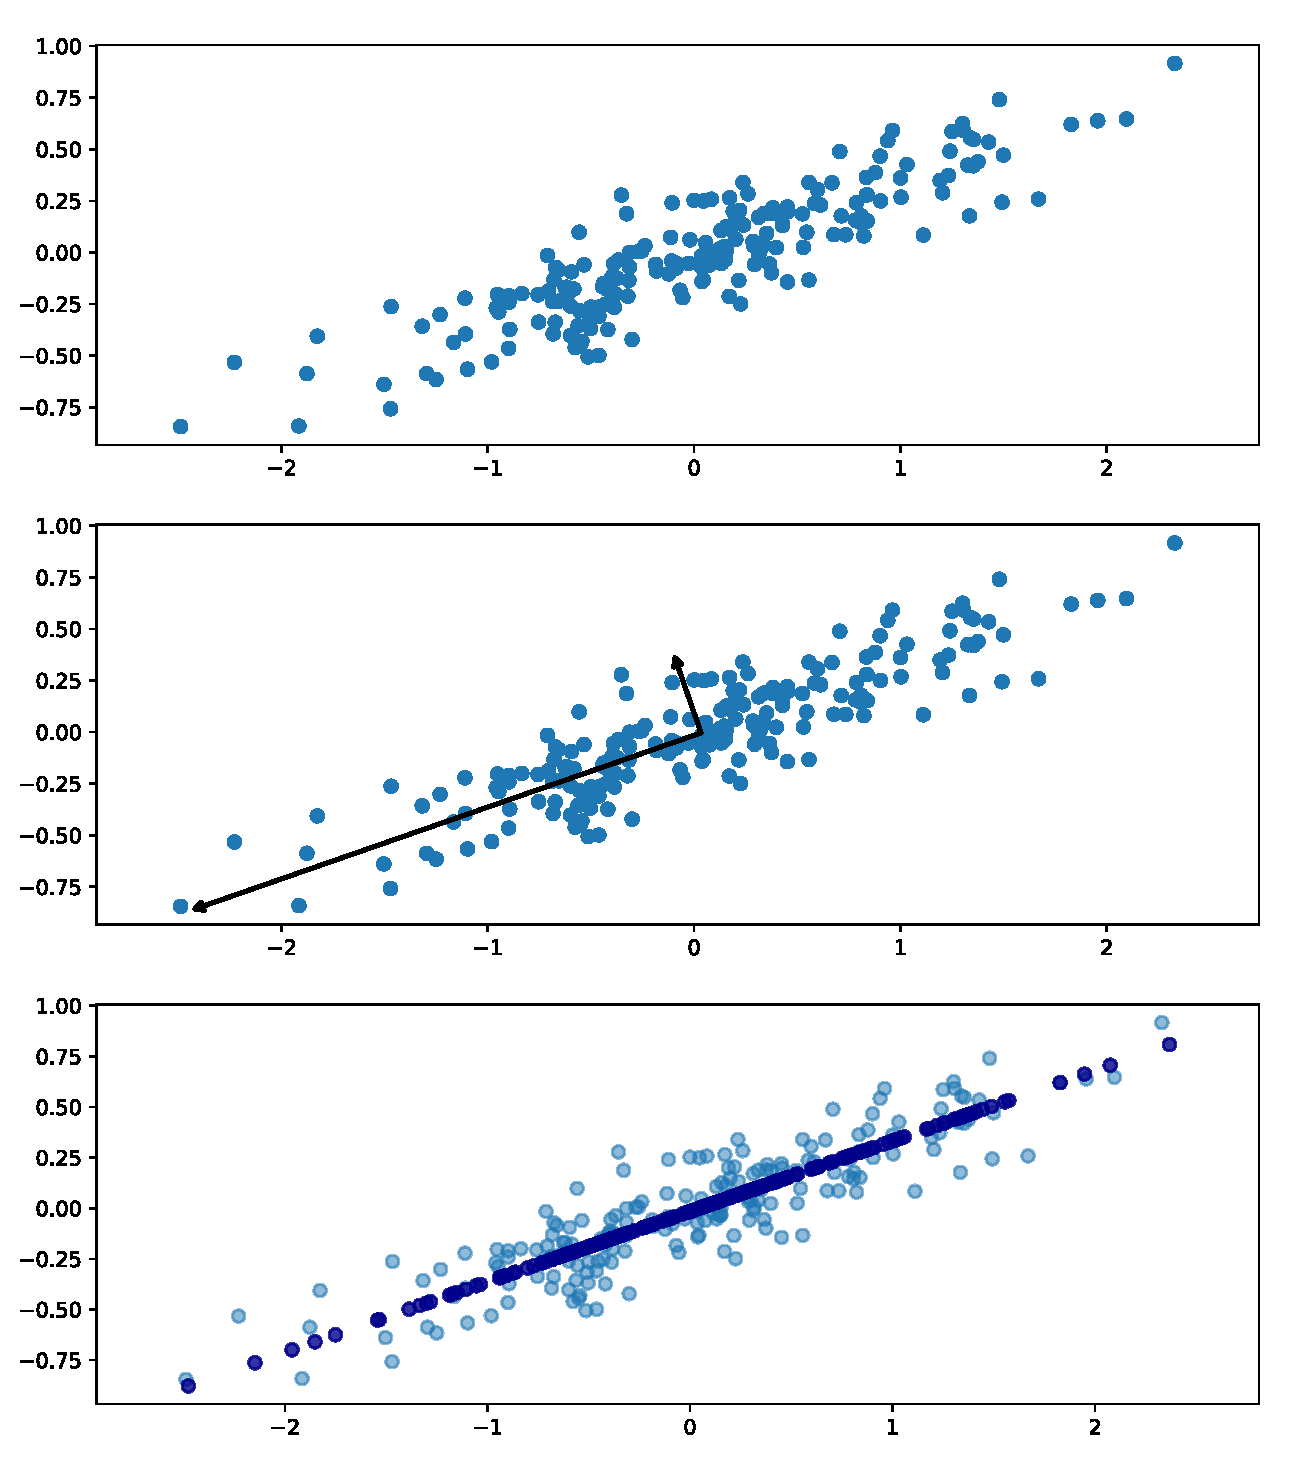
\includegraphics[width=15cm]{pca.pdf}
	\caption{Wizualizacja PCA na zbiorze punktów w przestrzeni dwuwymiarowej}
	\label{fig:pca}
\end{figure}

Wykres \ref{fig:pcacumsum} przedstawia zależność między ilością składników PCA a procentem wariancji opisywanym przez składniki na podstawie zbioru danych MNIST. Ilość składników mieści się w przedziale od 1 do 784 (28 razy 28 piksel). Jak można zauważyć, dane reprezentowane przez około 80 wartości są w stanie opisać 90\% wariancji danych, co jest znaczą redukcją z 784. Przy 400 składnikach osiągnięto praktycznie 100\% pokrycia. 
\begin{figure}[h!]
	\centering
	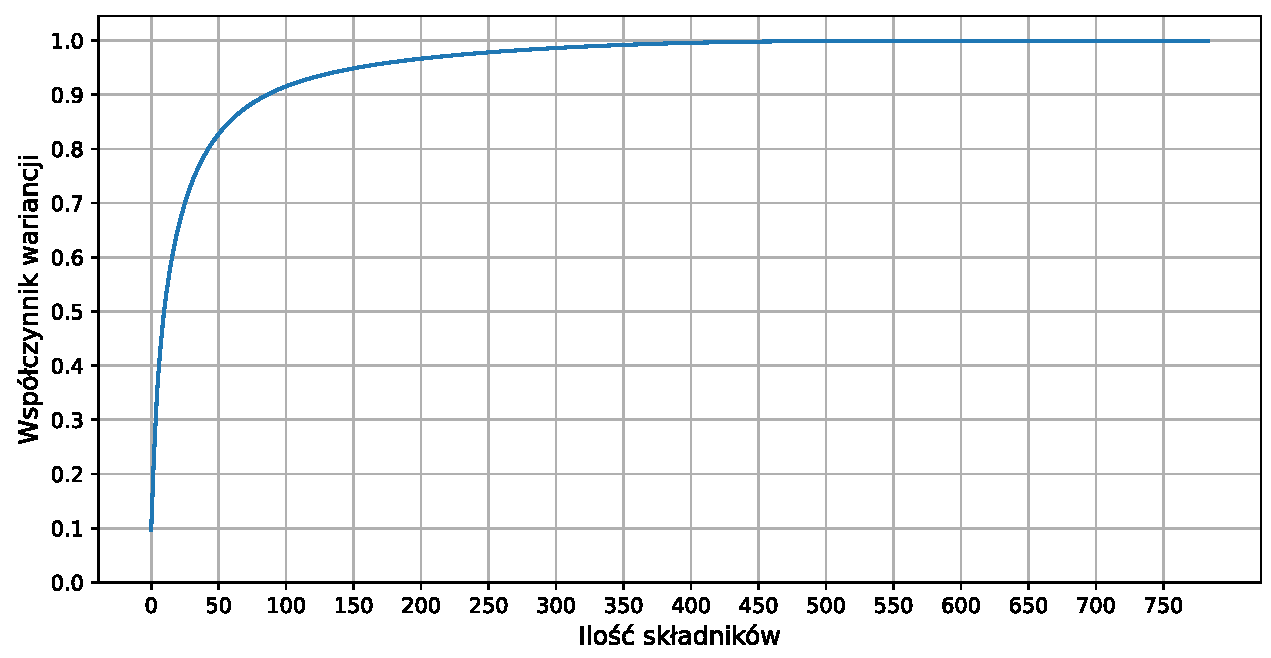
\includegraphics[width=\textwidth]{pcacumsum.pdf}
	\caption{Procent wariancji opisywany przez ilość składników}
	\label{fig:pcacumsum}
\end{figure}



Użycie autoenkodera jest jedną z możliwości dokonania redukcji wymiarów. Jego budowa wymusza naukę jak najlepszej reprezentacji danych w zadanej długości kodu. Zadaniem enkodera jest zachowanie w zmiennych jak najwięcej informacji dotyczących wejścia, a dekodera -- odwzorowanie jak najwięcej z nich. Najważniejszą cechą autoenkodera jest możliwość nauki przekształceń zarówno liniowych, jak i nieliniowych w zależności od doboru funkcji aktywacji. Różnicę pomiędzy oboma przekształceniami pokazano na rysunku \ref{fig:pcavsautoenkoder} \cite{nonlinearpca}.
\begin{figure}[h!]
	\centering
	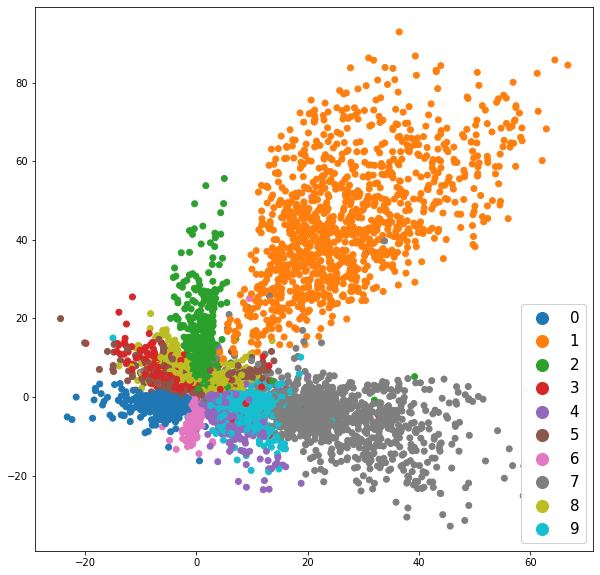
\includegraphics[width=10.5cm]{pictures/aelatentspace.png}
	\caption{Przestrzeń dwuwymiarowej zmiennej ukrytej dla zbioru MNIST}
	\label{fig:latentspaceae}
\end{figure}

\subsubsection{Analiza zastosowanych metod}
Przedstawione metody są często wykorzystywane w problemach redukowania wymiarów. Wybór jednej z nich powinien zostać dopasowany do potrzeb i do zbioru danych, który jest używany. PCA, będąc ograniczone do jedynie liniowych przekształceń, jest szybsze niż autoenkoder, który wymaga treningu \cite{aevspca2}. Jest ono też lepszym wyborem, kiedy dane są nadmiernie skorelowane. Rozpatrując przykład zbioru danych opisującego takie cechy ludzi, jak wzrost, waga, kolor oczu oraz długość włosów, oczywiste jest, że czyjaś waga jest zależna od wzrostu. PCA w takim przykładzie bez problemu odnajdzie tą zależność i zredukuje. Autoenkoder jest lepszym wyborem, kiedy dane są o wiele bardziej złożone, czyli są to na przykład obrazy lub pliki audio.  
Jednowarstwowy autoenkoder z liniową funkcją aktywacji na każdej warstwie zachowuje się dokładnie tak samo jak PCA \cite{aevspca}.
\begin{figure}[h!]
	\centering
	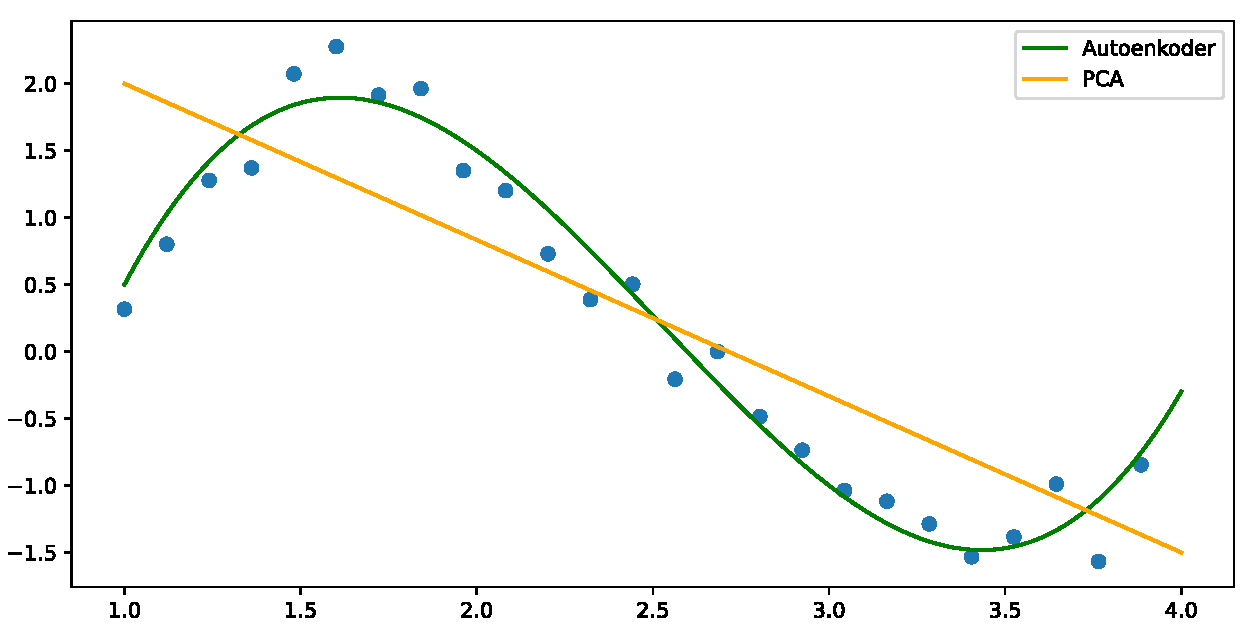
\includegraphics[width=14cm]{pcavsautoencoder.pdf}
	\caption{Liniowe oraz nieliniowe przekształcenie}
	\label{fig:pcavsautoenkoder}
\end{figure}

\subsection{Odszumianie obrazów}
Model autoenkodera przeznaczony do odszumiania danych często dostaje swoją nazwę i jest określany mianem \textit{Denoising autoencoder} (DAE). Tak jak zwykły autoenkoder, próbuje w jak najlepszy sposób skompresować dane, zachowując jak najwięcej istotnych informacji. Najważniejszą różnicą między tymi modelami są dane, które modele dostają na wejście i wyjście. Obrazy przyjmowane na warstwę wejściową są zaszumione, natomiast te z warstwy wyjściowej pochodzą prosto ze zbioru danych.
Powodem, dla którego autoenkodery tak dobrze nadają się do odszumiania, jest ich umiejętność kompresji danych. Kompresja, której dokonują te modele jest stratna. W przypadku, kiedy głównym zadaniem jest jak najlepsze odtworzenie danych wejściowych, staje się to problemem, jednak w tym przypadku można wykorzystać tę własność. Porównując wyjście modelu z danymi bez szumu, zapewniamy, że model nauczy się w jakimś stopniu odtwarzać je poprawnie. Zmusza to w ten sposób model do ignorowania nieistotnych części danych oraz zapamiętywanie tylko tych, na podstawie których będzie możliwe jak najlepsze odwzorowanie wejścia sieci.
Rysunek \ref{fig:noisedae} pokazuje możliwości modelu na przykładzie zbioru danych MNIST. Do obrazów przeznaczonych na trening został dodany szum. Zaszumiony obraz powstał przez dodanie do oryginalnego obrazu losowo wybranych wartości z rozkładu Gaussa $\mathcal{N}(0,1)$ przemnożonych przez stałą, która w tym przypadku wynosi $0,4$. Następnie obrazy wejściowe zostały skompresowane do kodu o długości 5, a następnie odkodowane przez dekoder. 
\begin{figure}[h!]
	\centering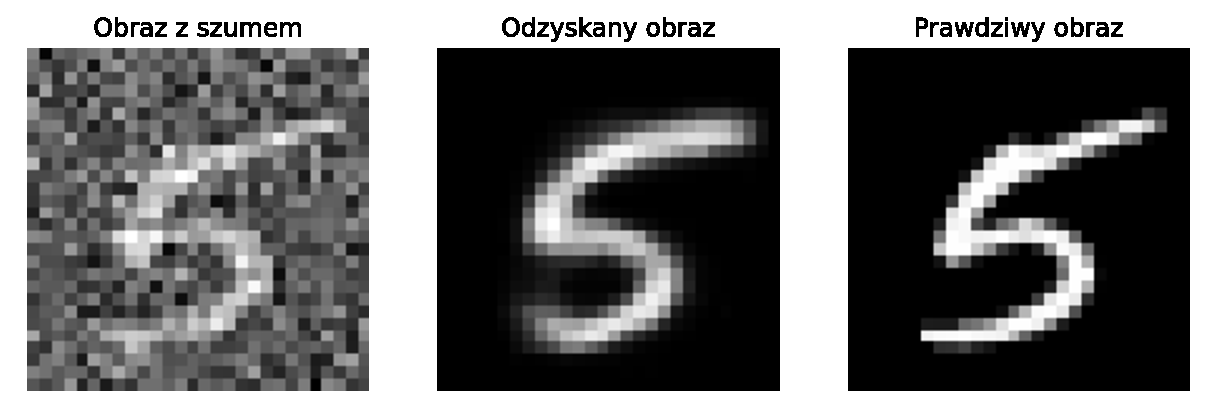
\includegraphics[width=14.5cm]{denoisingae.pdf}
	\caption{Obraz z szumem, odzyskany oraz prawdziwy}
	\label{fig:noisedae}
\end{figure}

Wadą autoenkodera przeznaczonego do odszumiania danych jest jego ścisłe powiązanie ze zbiorem danych, na których został wytrenowany. Model z parametrami wytrenowanymi na jednym zbiorze danych nie będzie nadawał się do innego zbioru, z którego danymi będzie pracował. Jedynym rozwiązaniem tego problemu jest stworzenie nowego modelu przeznaczonego do użytku na nowych danych. 
\subsection{Uzupełnianie obrazów}
Uzupełnianie obrazów ma na celu wypełnienie brakującej lub zamaskowanej części obszaru. Człowiek jest w stanie sobie poradzić z tym zadaniem bez problemu, jednak dla komputera nie jest ono oczywiste. Bierze się to z tego, że jest ogromna ilość możliwości wypełnienia nawet niewielkiej brakującej przestrzeni. 
Można wyróżnić dwa główne podejścia wypełniania obrazów:
\begin{itemize}
	\item sieć posiada informację, w którym miejscu obrazu jest luka;
	\item sieć musi sama się nauczyć, które miejsce obrazu musi wypełnić.
\end{itemize}
Rysunek \ref{fig:lukaae} przedstawia podejście do problemu, kiedy sieć nie wie, w którym miejscu znajduje się luka. 
\begin{figure}[h]
	\centering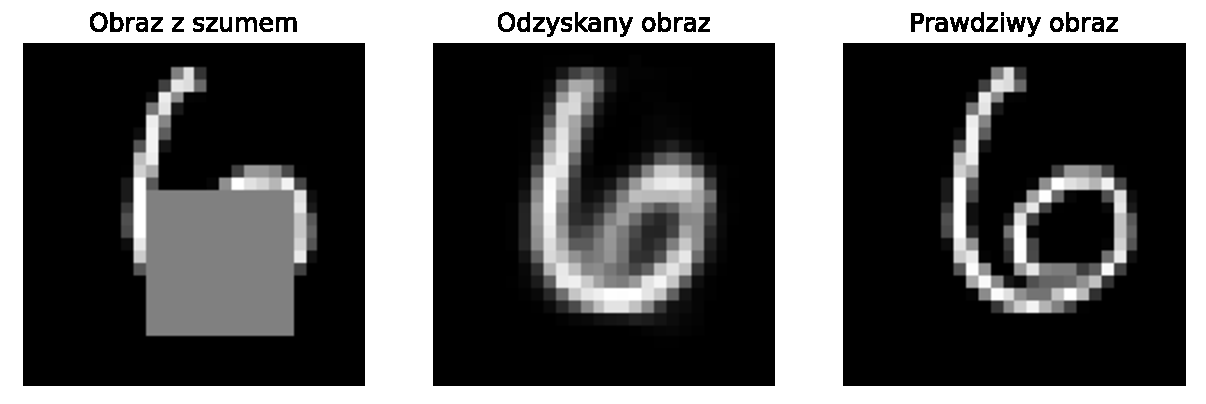
\includegraphics[width=14.5cm]{completionae.pdf}
	\caption{Obraz z luką, odzyskany oraz prawdziwy}
	\label{fig:lukaae}
\end{figure}

\section{Problemy z generacją nowych danych}
 Sieć neuronowa budująca dekoder jest w stanie po treningu ze zmiennych ukrytych odkodować zakodowany obraz. Ustawiając wejście dekodera na losowy punkt z przestrzeni zmiennych generowanych przez enkoder, powinno się otrzymać obraz, który jest podobny do tych, na których cała sieć została wytrenowana.
Aby model mógł generować nowe dane, muszą zostać spełnione dwa warunki:
\begin{itemize}
	\item Przestrzeń kodu (tzw. zmiennych ukrytych) musi być ciągła, co znaczy, że dwa punkty znajdujące się obok siebie będą dawać podobne dane, kiedy zostaną odkodowane.
	\item Przestrzeń musi być kompletna, co znaczy, że punkty wzięte z dystrybucji muszą dawać wyniki mające sens.
\end{itemize}
Tradycyjna architektura nie zapewnia przed treningiem żadnego z tych warunków. W dodatku nie znamy, jaka jest dystrybucja, według której enkoder wybiera zmienne. Na rysunku \ref{fig:latentspaceae}, widać, że przestrzeń zawiera niezdefiniowane punkty. Szczególnie dobrze to widać między klasami oznaczającymi cyfry jeden oraz siedem. Zadaniem modelu jest jak najlepsze odzwierciedlenie skompresowanych danych, a nie zapewnienie, czy rozkład zmiennych kodu spełnia przedstawione warunki. Może się zdarzyć, że sieć nauczy się pasującej dystrybucji, jednak jest to bardzo mało prawdopodobne. Chcąc zbudować model generacyjny, trzeba posiadać gwarancję, że za każdym razem rozkład będzie spełniał odpowiednie warunki.
\newpage
\section{Wnioski}
Autoenkodery jako zwyczajne sieci neuronowe o zwężonej budowie najlepiej sprawdzają się w problemach kompresji i rekonstrukcji danych. Kompresja wejścia modelu do kodu pozwala na zachowanie tylko najistotniejszych elementów, na podstawie których będzie można zrekonstruować je jak najlepiej. Zadania opierające się na tym procesie to między innymi: redukcja wymiarów, usuwanie szumu czy detekcji anomalii. Każdy ten przykład opiera się na tej samej zasadzie działania polegającej na kompresji. Model, porównując ze sobą dane wejściowe oraz te, które pochodzą z warstwy wyjściowej, jest w stanie po wielu epokach treningu zacząć generalizować. Pozwala to na ignorowanie elementów, które są nieistotne w odtwarzaniu danych wejściowych. Enkoder tradycyjnego autoenkodera nie kontroluje, według jakiej dystrybucji rozłożona jest przestrzeń kodu. Chcąc wygenerować nowe dane, nie wiadomo, które jej punkty będą w stanie wygenerować podobne dane, ponieważ przestrzeń kodu może posiadać przestrzenie niezdefiniowane.
 
\chapter{Autoenkodery wariacyjne}
\section{Informacje ogólne}
Wariacyjny autoenkoder (VAE) rozwiązuje problemy generacyjne tradycyjnego modelu. VAE ma na celu skompresowanie danych do określonego wielowymiarowego rozkładu ukrytego, a następnie z próbki tej dystrybucji próbuje jak najlepiej zrekonstruować wejście. Model ten należy go grupy wariacyjnych metod Bayesowskich, czemu zawdzięcza swoją nazwę. Dystrybucjami najczęściej wybieranymi do reprezentacji zmiennych ukrytych są rozkłady normalne. Rozkład normalny jest opisywany przy pomocy dwóch wartości: średnia, która oznaczana jest znakiem $\mu$ oraz odchylenie standardowe oznaczane $\sigma$. Jeśli dane zostaną skompresowane do kodu o długości $n$, enkoder wygeneruje dwa wektory $n$-wymiarowe, z którego jeden będzie przechowywał wartości średniej, a drugi odchylenia standardowego dla każdego z $n$ rozkładów normalnych co przedstawia rysunek \ref{fig:vaeschemat} \cite{vaetootorial}.
\begin{figure}[h!]
	\centering
	\begin{tikzpicture}
		\node (true) at (-6.5, 0) {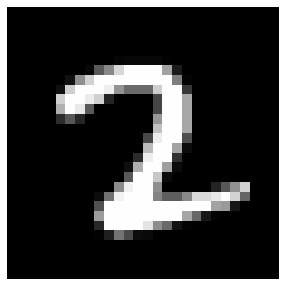
\includegraphics[width=2.5cm]{vaeorg1.png}};
		\draw[thick] (-4.6, 1) -- (-4.6, -1) node[pos=0.5] (enkoderin){} -- (-3.5, -0.6) -- (-3.5, 0.6) node[pos=0.5] (enkoderout){} -- cycle;
		\draw[-latex, thick] (true.east) -- (enkoderin.west);                                                                                 
		\node[scale=0.7](meanv) at (-2.5, 0) {\(\begin{bmatrix}                                                                                
		1.88 \\ 1.24 \\ \vdots \\ 2.09 \\ 2.18                                                                                        
		\end{bmatrix}\)};                                                                                                                     
		\node[scale=0.7] (stdv) at (-1.5, 0) {\(\begin{bmatrix}                                                                              
            0.34 \\ 0.92 \\ \vdots \\ 1.69 \\ 0.15                                                                        
			\end{bmatrix}\)};                                                                                                                    
		\draw[-latex, thick](enkoderout.east) -- (meanv.west);                                                                                 
		\node[scale=0.7] (nv) at (0.5, 0) {\(\begin{bmatrix}                                                                                  
				 \mathcal{N}(1.88,0.34)\\ \mathcal{N}(1.24,0.92) \\ \vdots \\ \mathcal{N}(2.09,1.69) \\ \mathcal{N}(2.18,0.15)
			\end{bmatrix}\)};
		\draw[-latex, thick] (stdv.east) -- (nv.west);
		\node[scale=0.7] (sample) at (2.5, 0) {\(\begin{bmatrix}
				1.28 \\ 1.87 \\ \vdots \\ 2.01 \\ 2.28
			\end{bmatrix}\)};
		\draw[-latex, thick] (nv.east) -- (sample.west);
				\draw[thick] (3.5, 0.6) -- (3.5, -0.6) node[pos=0.5] (dekoderin){} -- (4.6, -1) -- (4.6, 1) node[pos=0.5] (dekoderout){} -- cycle;
		\node (recon) at (6.5, 0) {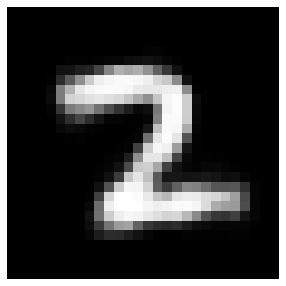
\includegraphics[width=2.5cm]{vaerec1.png}};
		\draw[-latex, thick](sample.east) -- (dekoderin.west);
		\draw[-latex, thick](dekoderout.east) -- (recon.west);
		% Labels
		\node at (-6.5, -1.5) {wejście};
		\node at (6.5, -1.5) {wyjście};
		\node at (-2.5, -1.5) {$\mu$};
		\node at (-1.5, -1.5) {$\sigma$};
		\node at (2.5, -1.5) {$z$};
		\node at (0.5, -1.5) {dystrybucje};
		\node at (-4.05, -1.5) {enkoder};
		\node at (4.05, -1.5) {dekoder};

	\end{tikzpicture}
	\caption{Schemat budowy wariacyjnego autoenkodera}
	\label{fig:vaeschemat}
\end{figure}
 
 Rozkład normalny spełnia warunki potrzebne dla modelu generacyjnego. Jego ciągłość i kompletność sprawia, że dekoder patrząc na obraz wyjściowy i porównując go z prawdziwym, nauczy się w bardzo podobny sposób odkodowywać niedaleko oddalone od siebie punkty należące do opisywanej dystrybucji.

\begin{figure}[h!]
	\centering
	\pgfplotsset{
		colormap={whitered}{color(0cm)=(white); color(1cm)=(orange!75!red)}
	}
	\begin{tikzpicture}[
		declare function={mu1=2;},
		declare function={mu2=3;},
		declare function={sigma1=0.5;},
		declare function={sigma2=0.6;},
		declare function={normal(\m,\s)=1/(2*\s*sqrt(pi))*exp(-(x-\m)^2/(2*\s^2));},
		declare function={bivar(\ma,\sa,\mb,\sb)=
			1/(2*pi*\sa*\sb) * exp(-((x-\ma)^2/\sa^2 + (y-\mb)^2/\sb^2))/2;}]
		\begin{axis}[
			colormap name=whitered,
			width=15cm,
			view={45}{55},
			enlargelimits=false,
			grid=major,
			domain=0:5,
			y domain=0:5,
			samples=31,
			xlabel=$x_2$,
			ylabel=$x_1$,
			zlabel={$P$},
			]
			\addplot3 [surf] {bivar(mu1,sigma1,mu2,sigma2)};
			\addplot3 [domain=0:5,samples=31, samples y=0, thick, smooth] (x,5,{normal(mu1,sigma1)});
			\addplot3 [domain=0:5,samples=31, samples y=0, thick, smooth] (0,x,{normal(mu2,sigma2)});
			
			\draw [black!50] (axis cs:-1,0,0) -- (axis cs:4,0,0);
			\draw [black!50] (axis cs:0,-1,0) -- (axis cs:0,4,0);
			
			\node at (axis cs:0,2,0.12) [pin=165:$P(x_1)$] {};
			\node at (axis cs:4,4,0.32) [pin=-15:$P(x_2)$] {};
		\end{axis}
	\end{tikzpicture}
	\caption{Wielowymiarowy rozkład zmiennej ukrytej}
\end{figure}
\begin{figure}[h!]
	\centering
	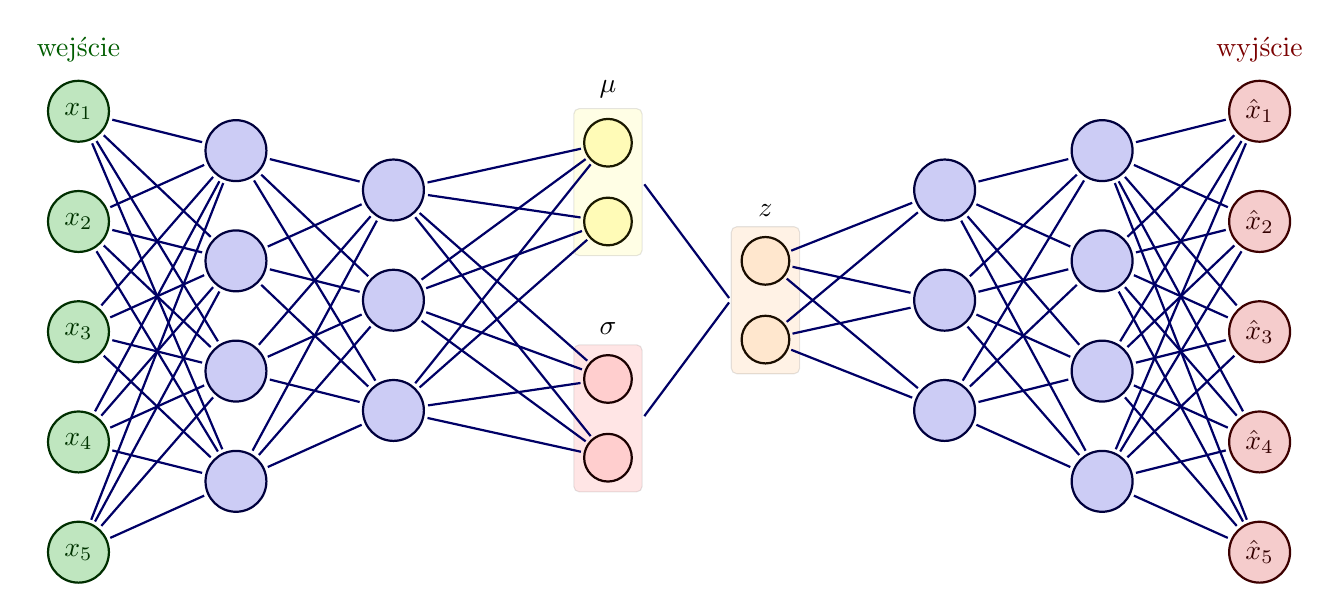
\begin{tikzpicture}[
		shorten >=1pt, shorten <=1pt,
		neuron/.style={circle, draw, minimum size=4ex, thick},
		hidden/.style={node,blue!20!black,draw=myblue!30!black,fill=myblue!20},
		myin/.style={node,green!20!black,draw=mygreen!30!black,fill=mygreen!25},
		myout/.style={node,red!20!black,draw=myred!30!black,fill=myred!20},
		legend/.style={font=\large\bfseries},
		]
		
		% encoder
		\drawEncoder{encoder}{{{,,,,}, {,,,}, {,,}}}
		\denselyConnectNodes{encoder}{{5, 4, 3}}
		
		% decoder
		\begin{scope}[xshift=11cm]
			\drawDecoder{decoder}{{{,,}, {,,,}, {,,,,}}}
			\denselyConnectNodes{decoder}{{3, 4, 5}}
		\end{scope}
		
		% mu, sigma, sample nodes
		\foreach \idx in {1,...,2} {
			\coordinate[neuron, right=2 of encoder-3-2, yshift=\idx cm, fill=yellow, fill opacity=0.2] (mu-\idx);
			\coordinate[neuron, right=2 of encoder-3-2, yshift=-\idx cm, fill=red, fill opacity=0.1] (sigma-\idx);
			\coordinate[neuron, right=4 of encoder-3-2, yshift=\idx cm-1.5cm, fill=orange, fill opacity=0.1] (sample-\idx);
		}
		
		% mu, sigma, sample boxes
		\node [label=$\mu$, fit=(mu-1) (mu-2), draw, fill=yellow, opacity=0.1, rounded corners=2] (mu) {};
		\node [label=$\sigma$, fit=(sigma-1) (sigma-2), draw, fill=red, opacity=0.1, rounded corners=2] (sigma) {};
		\node [label=$z$, fit=(sample-1) (sample-2), draw, fill=orange, opacity=0.1, rounded corners=2] (sample) {};
		
		% mu, sigma, sample connections
		\draw[connect] (mu.east) edge (sample.west) (sigma.east) -- (sample.west);
		\foreach \a in {1,2,3}
		\foreach \b in {1,2} {
			\draw[connect] (encoder-3-\a) -- (mu-\b);
			\draw[connect] (encoder-3-\a) -- (sigma-\b);
			\draw[connect] (sample-\b) -- (decoder-1-\a);
		}
		
		\node[above=0.1 of encoder-1-1,mygreen!60!black] {wejście};
		\node[above=0.1 of decoder-3-1,myred!60!black] {wyjście};
		
	\end{tikzpicture}
	\caption{Sieć neuronowa tworząca VAE}
	\label{fig:vaenetwork}
\end{figure}

Sieć neuronowa budująca wariacyjny autoenkoder posiada dość nietypową budowę. Ostatnia ukryta warstwa enkodera łączy się z dwiema niepołączonymi ze sobą warstwami reprezentującymi średnią oraz odchylenie standardowe normalnej dystrybucji, której enkoder chce się nauczyć. Obie warstwy łączą się w jedną, która dokonuje losowania punktu z dystrybucji na nauczonych parametrach. Warstwy reprezentujące średnią $\mu$, odchylenie standardowe $\sigma$ oraz zmienne ukryte $z$ muszą posiadać taką samą liczbę neuronów przedstawiającą długość wektora reprezentującego skompresowane dane.
\section{Matematyczna definicja VAE}
Wariacyjny autoenkoder mimo swojego podobieństwa do tradycyjnego modelu znacznie różni się w opisie matematycznym. Największe różnice są obserwowane w definicji enkodera. Kod, który on produkuje, nazywany jest wartościami ukrytymi, ponieważ są one wnioskowane na podstawie każdej danej. Trenując tradycyjny model, nie jest istotna dystrybucja $p(z|x)$, z której pochodzą zmienne. Enkoder wariacyjnego autoenkodera jest zobowiązany do nauki konkretnej dystrybucji. Wyrażenie $p(z|x)$ jest rozumiane jako dystrybucja generująca zmienne ukryte na podstawie przedstawionej danej $x$. Należy wyznaczyć ten rozkład. Używając twierdzenie Bayesa wiadomo, że:
\begin{equation}
	p(z|x)=\dfrac{p(x|z)p(z)}{p(x)}
	\label{bayes}
\end{equation}
Rozkład marginalny $p(x)$ można zapisać w następujący sposób:
\begin{equation}
	p(x) = \displaystyle\int_{z}^{}p(x|z)p(z)dz
	\label{pxcalka}
\end{equation}
Obliczenie tej całki jest bardzo trudne lub nawet obliczeniowo niemożliwe w rozsądnym czasie, ponieważ $z$ jest często wielowymiarowym wektorem, a trzeba całkować po wszystkich wymiarach. Aby próbować policzyć tę całkę w inny sposób, można wybrać jedną z dwóch metod:
\begin{itemize}
	\item próbkowanie Monte Carlo łańcuchami Markowa;
	\item wnioskowanie wariacyjne.
\end{itemize}
Przestrzeń przeszukiwań może być kombinatorycznie za duża, aby korzystać z pierwszej metody lub błąd przybliżenia tej całki będzie za duży w przypadku znacznej ilości wymiarów \cite{salimans2015markov}.

\section{Wnioskowanie wariacyjne}
Wnioskowanie wariacyjne pozwala zastąpić jedną dystrybucję, która nie jest bezpośrednio znana na taką, jaka pasuje do problemu oraz dobrze odzwierciedla rozkład początkowy \cite{variationalinference}. Używając tej metody, uda się rozwiązać problem wyznaczenia rozkładu $p(z|x)$. Zastąpiony będzie rozkładem $q$, który jak najlepiej odwzoruje oryginalny rozkład. 

Wykres \ref{fig:app} przedstawia dwie krzywe. Pomarańczowa krzywa opisująca rozkład normalny zastępuje w optymalny sposób prawdziwą dystrybucję oznaczoną kolorem niebieskim.
\begin{figure}[h!]
	\centering
	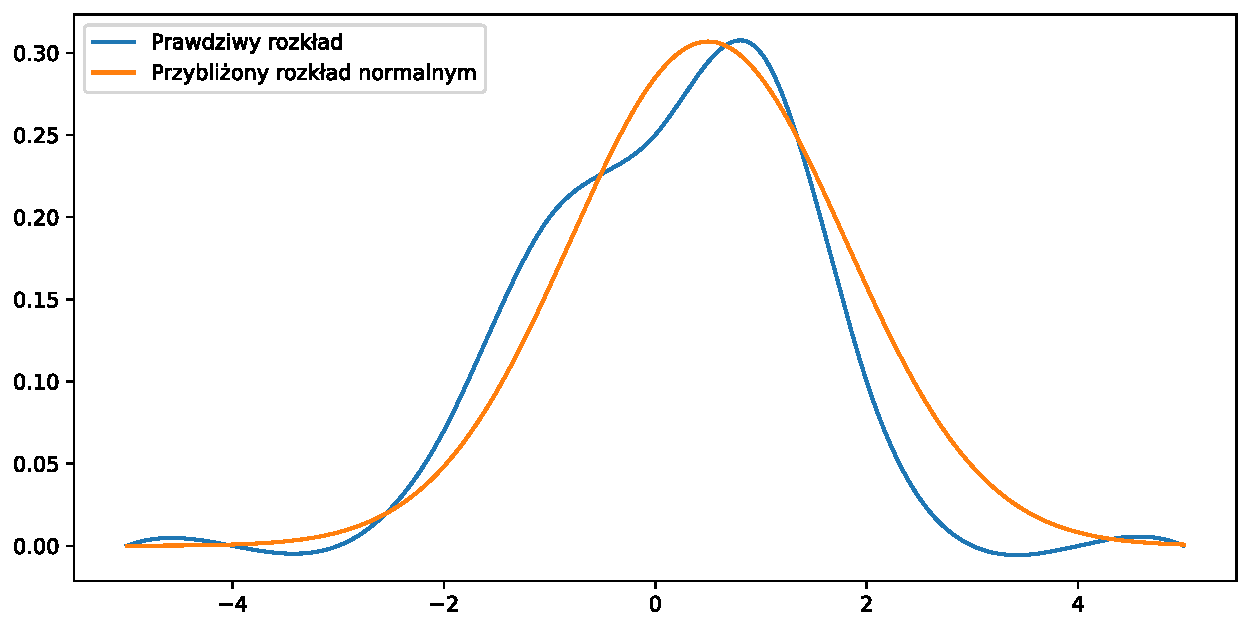
\includegraphics[width=12cm]{approximate.pdf}
	\caption{Prawdziwa oraz przybliżona dystrybucja}
		\label{fig:app}
\end{figure} 

\subsection{Dywergencja Kullbacka-Leiblera}
Aby zminimalizować błąd pomiędzy prawdziwą a zamienną dystrybucją, należy posiadać miarę, która określa rozbieżność między dwoma rozkładami prawdopodobieństwa. Miarą tą jest dywergencja Kullbacka-Leiblera ($D_{KL}$). Podstawowymi jej własnościami są:
\begin{itemize}
	\item jej wartość jest nieujemna; $D_{KL}(P\|Q)) \geq 0$. Miara przyjmuje wartość 0 tylko w przypadku, kiedy $P$ i $Q$ są identycznymi dystrybucjami;
	\item miary tej nie można określić mianem metryki, ponieważ nie jest symetryczna ($D_{KL}(P\|Q)\neq D_{KL}(Q\|P)$);
\end{itemize}
Celem jest zminimalizowanie błędu, co sprawi, że rozkład $q(z|x)$ będzie jak najbardziej podobny do $p(z|x)$:
\begin{equation}
	q^\ast(z|x)=\operatorname*{argmin}_{q(z|x)\in Q}(D_{KL}(q(z|x)\|p(z|x)))\\
		\label{qopt}
\end{equation}
gdzie $Q$ to rodzina prostych dystrybucji, na przykład rozkładów Gaussa.
\subsection{Dolna granica dowodów}
Dywergencja jest określana jako:
\begin{equation}
	D_{KL}(q(z|x)\|p(z|x))=\displaystyle\int_{z}^{}q(z|x)\log\frac{q(z|x)}{p(z|x)}dz
	\label{kld1}
\end{equation}
Wyznaczenie $q(z|x)$ jest proste, ponieważ sami dobieramy, jaką dystrybucją jest $q$. Dla modelu VAE najczęściej jest to rozkład normalny. Mimo to obliczenia nie są możliwe, ponieważ znowu występuje problem wyznaczenia $p(z|x)$. Tym razem można przepisać:
\begin{equation}
	p(z|x)=\dfrac{p(x,z)}{p(x)}
	\label{bayesinaczej}
\end{equation}
Podstawiając zapisaną inaczej wartość $p$ do wzoru na dywergencję, otrzymuje się \cite{filmik1}:
\begin{equation}
	D_{KL}(q(z|x)\|p(z|x))=\displaystyle\int_{z}^{}q(z|x)\log\frac{q(z|x)}{p(x,z)}p(x)dz
	\label{kldlogarytmy}
\end{equation}
Własności logarytmów pozwalają zamienić iloczyn pod logarytmem na sumę w następujący sposób:
\begin{equation}
	D_{KL}(q(z|x)\|p(z|x))=\displaystyle\int_{z}^{}q(z|x)\left( \log\frac{q(z|x)}{p(x,z)} + \log p(x)\right) dz
	\label{kldcalka}
\end{equation}
Mnożąc $q(z|x)$ przez nawias, otrzymuje się sumę pod całką, którą można zapisać jako sumę dwóch całek. Następnie wartość $\log p(x)$ jest wyłączana przed całkę, ponieważ całkując po $z$, jest ona traktowana jako stała.
\begin{equation}
	D_{KL}(q(z|x)\|p(z|x))=\displaystyle\int_{z}^{}q(z|x)\left( \log\frac{q(z|x)}{p(x,z)}\right)dz + \log p(x)\underbrace{\displaystyle\int_{z}^{}q(z|x)dz}_{\text{$\alpha$}}
	\label{calkaalpha}
\end{equation}
Wartość całki oznaczonej jako $\alpha$ jest równa 1, dlatego, że $q$ jest funkcją dystrybucji prawdopodobieństwa oraz jest ona liczona po wszystkich zmiennych $z$.
\begin{equation}
	D_{KL}(q(z|x)\|p(z|x))=\underbrace{\displaystyle\int_{z}^{}q(z|x)\left( \log\frac{q(z|x)}{p(x,z)}\right)dz}_{\text{$\mathcal{L}$}} + \log p(x)
	\label{kldfinal}
\end{equation}
Wyprowadzony wzór można przepisać w następujący sposób:
\begin{equation}\label{elbo}
	\begin{array}{rcl}
		D_{KL}(q(z|x)\|p(z|x))= \mathcal{L} + \log p(x)\\[1ex]
	-\mathcal{L} = \log p(x) - D_{KL}(q(z|x)\|p(z|x))
	\end{array}
\end{equation}
Wartość $\log p(x)$ nosi nazwę dowodu, ponieważ mówi o prawdopodobieństwie otrzymania obserwacji $x$ przez model.
Parametr $-\mathcal{L}$ jest nazywany dolną granicą dowodu \textit{Evidence Lower BOund, ELBO}. Nazwa pochodzi od własności mówiącej o tym, że jej wartość jest zawsze mniejsza lub równa dowodowi. Własność ta bierze się z faktu, że dywergencja jest zawsze nieujemna.
\begin{center}
	$-\mathcal{L}\leq\log p(x)$
\end{center}
Wartość dowodu jest stała dla podanego $z$, więc problem minimalizacji dywergencji można zapisać jako:
\begin{equation}
	\operatorname*{argmin}D_{KL}(q(z|x)\|p(z|x)) = \operatorname*{argmin}\mathcal{L} = \operatorname*{argmax}-\mathcal{L}
	\label{equ:argmindkl}
\end{equation}
\subsection{Funkcja straty}
Korzystając z twierdzenia Bayesa zapisanego w \ref{bayesinaczej} można przepisać $\mathcal{L}$ jako:
\begin{equation}
	\begin{aligned}
		\mathcal{L}=\displaystyle\int_{z}^{}q(z|x)\left( \log\frac{q(z|x)}{p(x,z)}\right)dz=\\[1ex]
		\displaystyle\int_{z}^{}q(z|x)\left( \log\frac{q(z|x)}{p(x|z)p(z)}\right)dz
		\label{equ:kldlogagn}
	\end{aligned}
\end{equation}
Wykorzystując kolejny raz własności logarytmów, przekształcono:
\begin{equation}
	\mathcal{L}=\displaystyle\int_{z}^{}q(z|x)\log\frac{q(z|x)}{p(z)}dz - \displaystyle\int_{z}^{}q(z|x)\log\frac{q(z|x)}{p(x|z)}dz
	\label{equ:elbolog}
\end{equation}
Interpretując poszczególne składniki, $\mathcal{L}$ jest zapisywane jako:
\begin{equation}
	\mathcal{L} =  D_{KL}(q(z|x)\|p(z)) - \mathbb{E}_{z\sim q(z|x)}\log p(x|z)
	\label{equ:ostatniejuz}
\end{equation}
Równanie \ref{equ:argmindkl} pokazuje, że minimalizacja pierwotnej dywergencji oznacza również minimalizację $\mathcal{L}$. 

Pierwsze wyrażenie reprezentuje odległość pomiędzy dystrybucją zastępującą $p(z|x)$, czyli dystrybucją nauczoną przez enkoder a $p(z)$, czyli rozkładem zmiennych ukrytych, który sami wybierany. Drugie wyrażenie to wartość oczekiwana logarytmu prawdopodobieństwa otrzymania obserwacji $x$ z wartości ukrytych wybieranych z dystrybucji $q(z|x)$, której nauczył się enkoder.

Enkoder, jak i dekoder są zapisywane jako rozkłady prawdopodobieństwa. Funkcja $q(z|x)$ mówi, jakie zmienne ukryte $z$ reprezentują daną $x$, natomiast $p(x|z)$ generuje dane na podstawie otrzymanego kodu. Zapis $q(z|x)$ oznacza dystrybucję enkodera, a $p(x|z)$ -- dekodera.

Wariacyjny autoenkoder poruszany w pracy generuje zmienne ukryte z rozkładu normalnego $p(z)=\mathcal{N}(0,1)$. Przepuszczając wszystkie dane $x$ przez enkoder, wiemy, że próbkowane wartości przekazywane następnie do dekodera będą rozłożone normalnie. Rozwiązuje to problem tradycyjnego autoenkodera, którego zmienne ukryte są rozrzucone w sposób, który nie jest znany przed treningiem. Znając już dystrybucję, można policzyć dywergencję pomiędzy dwoma rozkładami normalnymi.
\begin{equation}
	\dfrac{1}{2}\displaystyle\sum_{D}^{i=1}\left\{\left(\dfrac{\sigma_0}{\sigma_1}\right)^2+\dfrac{(\mu_1 - \mu_0)^2}{\sigma_1^2} - 1 + 2\log\dfrac{\sigma_1}{\sigma_0}\right\}
	\label{equ:kldnormals}
\end{equation}
W przypadku, gdzie $\mu_1 = 0$ oraz $\sigma_1=1$ uprości się do \cite{kingma2014autoencoding}:
\begin{equation}
	\dfrac{1}{2}\displaystyle\sum_{D}^{i=1}\sigma_i^2+\mu_i^2-2\log(\sigma_i)-1
	\label{equ:kld_loss}
\end{equation} 
%\begin{center}
%	gdzie $D$ to długość wektora zmiennych ukrytych.
%\end{center}
gdzie $D$ to długość wektora zmiennych ukrytych. Jest to pierwsza część funkcji straty. 

Druga część funkcji straty jest nazywana błędem rekonstrukcji. Można zastąpić wartość oczekiwaną wartością jednej próbki, ponieważ do trenowania wag modeli używana jest metoda gradientu stochastycznego. Aby uniknąć liczenia skomplikowanych dystrybucji prawdopodobieństwa $\log p(x|z)$, gdzie poszczególne wymiary $x$ są zależne od siebie, liczy się proste rozkłady na każdym wymiarze osobno. Aby to osiągnąć, używa się binarnej entropii krzyżowej. W praktyce często są stosowane również inne funkcje, takie jak błąd średniokwadratowy, będący bardziej intuicyjnym rozwiązaniem.
Można tak zrobić, ponieważ wartość prawdopodobieństwa należy do przedziału $\left[ 0, 1\right] $, więc ujemny logarytm z małej liczby (słabego odwzorowania wejścia przez dekoder) będzie ogromną liczbą, a z bliskiej jedynki -- małą. W ten sam sposób również zachowuje się średni błąd kwadratowy. Aby lepiej kontrolować trening modelu, można balansować obie części funkcji straty, mnożąc poszczególne wartości przez wybrane stałe, aby model zachowywał się w dokładnie taki sposób, jak zostanie to zaplanowane \cite{balancing}.
%\newpage
\subsection{Metoda reparametryzacyjna}
Wariacyjny autoenkoder po zakodowaniu wejścia dokonuje operacji próbkowania (\textit{sampling}) z dystrybucji na nauczonych parametrach. Przy propagacji do przodu nie jest to problem, jednak podczas propagacji wstecznej jest to niemożliwe. Operacja losowania nie jest różniczkowalna, co sprawia, że nie można policzyć gradientu, który jest potrzebny do znajdowania minimalnej wartości funkcji straty. Sposobem obejścia tego problemu jest zastosowanie metody potocznie nazywanej sztuczką (\textit{reparameterization trick}) \cite{sztuczka}. Próbkowanie z dystrybucji $z\sim\mathcal{N}(\mu, \sigma)$ można zapisać jako:
\begin{center}
	$\epsilon\sim\mathcal{N}(0,1)$\\
	$z=\mu+\sigma\bigodot\epsilon$
\end{center} 
Pozornie nic się nie zmieniło, jednak teraz gradient jest przeprowadzany przez $z$, idąc od dekodera do enkodera, które jest teraz deterministyczne, co widać na grafice \ref{sztuczka} \cite{cokolwiek}. W poprzednim przypadku było ono losowo wybierane z dystrybucji. \\
\begin{figure}[h!]
	\centering
	\begin{tikzpicture}
		\node (dc) at (-4,0) {Dekoder};
		\node[shape=circle, draw=black, scale=1.2] (z) at (-4,-2) {$z$};
		\node (q) at (-2.6,-2) {$\sim q(z|x)$};
		\node[shape=diamond, draw=black] (sigma) at (-4,-4) {$\sigma$};
		\node[shape=diamond, draw=black] (mu) at (-6, -4) {$\mu$};
		\node (en) at (-5, -6) {Enkoder};
		
		\path[->] (z) edge node[left] {} (dc);
		\path[->] (mu) edge node[left] {} (z);
		\path[->] (sigma) edge node[left] {} (z);
		\draw[-to](-5, -5.5) -- (-5, -4.5);
		
		\node (dc1) at (4,0) {Dekoder};
		\node[shape=diamond, draw=black] (z1) at (4,-2) {$z$};
		\node (q1) at (6,-2) {$z=\mu+\sigma\bigodot\epsilon$};
		\node[shape=diamond, draw=black] (sigma1) at (4,-4) {$\sigma$};
		\node[shape=diamond, draw=black] (mu1) at (2, -4) {$\mu$};
		\node (en1) at (3, -6) {Enkoder};
		\node[shape=circle, draw=black, scale=1.2] (epsilon) at (6, -4) {$\epsilon$};
		\node (n) at (7.5, -4) {$\sim\mathcal{N}(0,1)$};
		
		\path[->] (z1) edge node[left] {} (dc1);
		\path[->] (mu1) edge node[left] {} (z1);
		\path[->] (sigma1) edge node[left] {} (z1);
		\path[->] (epsilon) edge node[left] {} (z1);
		\draw[-to](3, -5.5) -- (3, -4.5);
		
		\draw[-to](-1.5, -2) -- (2, -2) node[midway, above]{Reparametryzacja};
		
		\node[shape=diamond, draw=black, scale=1.2] (legend-diamond) at (-6, -7) {};
		\node[shape=circle, draw=black, scale=1.4] (legend-circle) at (-6, -8) {}; 
		\node (determin) at (-3, -7) {- węzeł deterministyczny};
		\node (randnode) at (-3.94, -8) {- węzeł losowy};
	\end{tikzpicture}
	\caption{Graficzna reprezentacja reparametryzacji}
	\label{sztuczka}
\end{figure}
\section{Zastosowania}
Wariacyjny autoenkoder jako pochodna tradycyjnego modelu może zostać zastosowany do takich samych zadań, jak detekcja anomalii, odszumianie oraz kompresja danych. Głównym jednak powodem, dla którego używa się modelu VAE, jest jego możliwość generowania danych. Mając już znaną dystrybucję, z której są losowane zmienne ukryte, aby generować nowe dane podobne do oryginalnych ze zbioru danych, należy podać jej losowy punkt na wejście do dekodera. Rysunek \ref{fig:vaelatent} przestawia zmienne ukryte wygenerowane przez enkoder dla obrazków z MNIST. Porównując obrazek \ref{fig:vaelatent} z \ref{fig:latentspaceae} widać, że model VAE rozwiązał omówione problemy generacyjne tradycyjnego autoenkodera. Przestrzeń jest kompletna i ciągła oraz nie zawiera przestrzeni niezdefiniowanych. Punkty dystrybucji znajdujące się blisko siebie generują podobne wyniki, co widać na obrazku \ref{fig:vaelatentgen}. Tak jak zostało założone, zmienne ukryte są rozłożone względem rozkładu normalnego. 

\begin{figure}[h!]
	\centering
	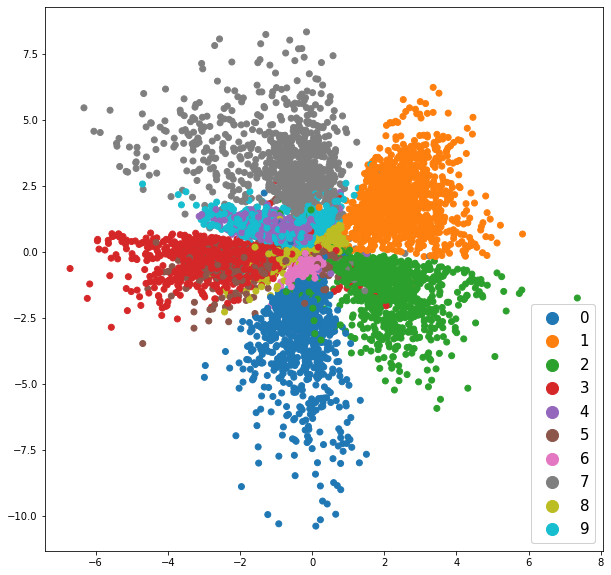
\includegraphics[width=12cm]{vaelatentspace.png}
	\caption{Przestrzeń zakodowanych zmiennych VAE}
	\label{fig:vaelatent}
\end{figure}
Obrazek \ref{fig:vaegeneracja} po lewej stronie pokazuje przykładowe dane ze zbioru danych MNIST, a prawa strona pokazuje dane wygenerowane przez wytrenowany model. Generując dane, nie potrzeba już enkodera. Na wejście dekoder dostaje losowo wybrane punkty z dystrybucji, którą wybiera się podczas budowy modelu. W tym przypadku jest to rozkład normalny.
\newpage
\begin{figure}[h!]
	\centering
	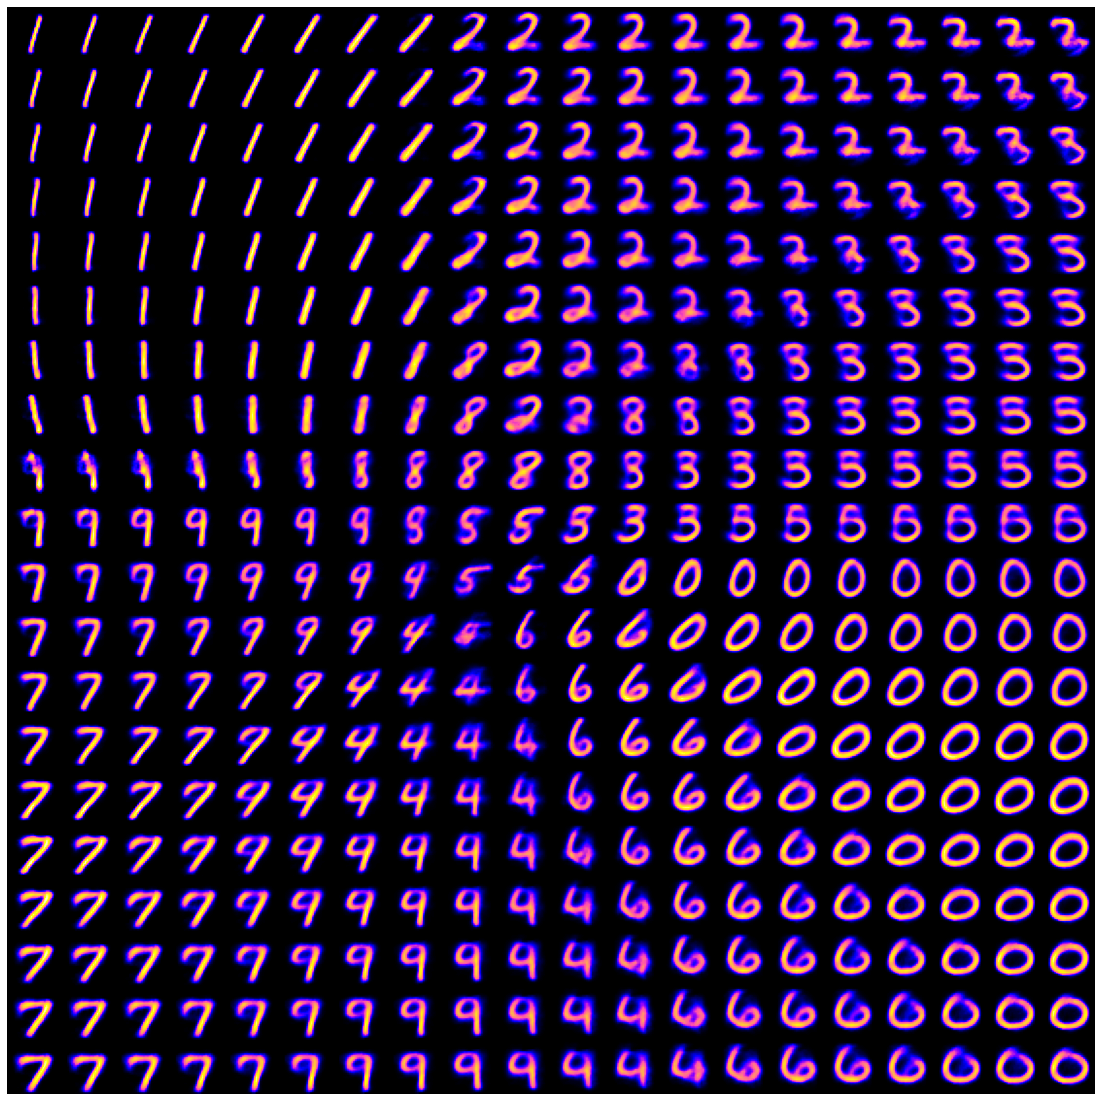
\includegraphics[width=14cm]{vaelatentgen.png}
	\caption{Wygenerowane obrazy przez VAE na przestrzeni zmiennych}
	\label{fig:vaelatentgen}
\end{figure}

\begin{figure}[h!]
	\centering
	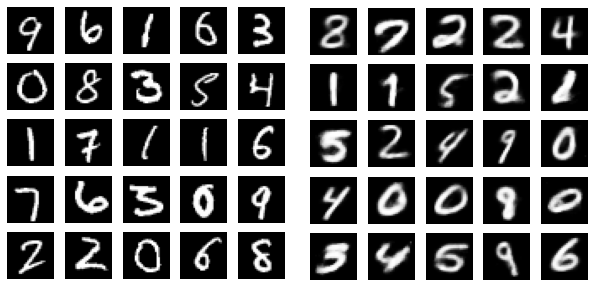
\includegraphics[width=12cm]{vaegeneracja.png}
	\caption{Porównanie prawdziwych oraz wygenerowanych obrazów}
	\label{fig:vaegeneracja}
\end{figure}

\subsection{Generacja ludzkich twarzy}
Zbiór danych \textit{CelebFaces Attributes Dataset (CelebA)} jest zbiorem ponad 200 000 twarzy celebrytów opisanych przez 40 atrybutów \cite{celeba}. Wymiary każdego obrazu to 178 na 218 pikseli. Na podstawie zbioru zostaną zaprezentowane możliwości generacyjne modelu VAE. Obrazom przeznaczonym do treningu sieci zostały obcięte brzegi, zostawiając obraz o wymiarach 120 na 120 pikseli, co poprawia wydajność modelu poprzez zostawienie tylko twarzy celebryty bez zbędnych informacji z tła.

Architekturą wykorzystywaną w tym problemie jest konwolucyjny wariacyjny autoenkoder (\textit{CVAE}). Sieci konwolucyjne wchodzące w skład enkodera wyjątkowo dobrze nadają się do pracy z obrazami \cite{convvae}. Obrazy zostały zakodowane do rozkładu o wymiarze 1024. Na rysunku \ref{fig:convvae} kolorem żółtym zostały oznaczone warstwy konwolucyjne, a ich poszczególne parametry i funkcje aktywacji zostały opisane pod nimi. W zwężeniu warstwa \textit{flatten} pozwala przejść z trójwymiarowych warstw na jeden wymiar, co umożliwia spłaszczenie obrazów do ukrytych rozkładów. Następnie po operacji losowania w warstwie $z$ wartości przechodzą do warstwy głębokiej mającej taki sam wymiar jak warstwa \textit{flatten}. \textit{Reshape} zamienia z powrotem wartości jednowymiarowe na trójwymiar, przez co warstwy dekonwolucyjne, oznaczone na zielono, mogą odkodować obraz.

\begin{figure}[h!]
	\centering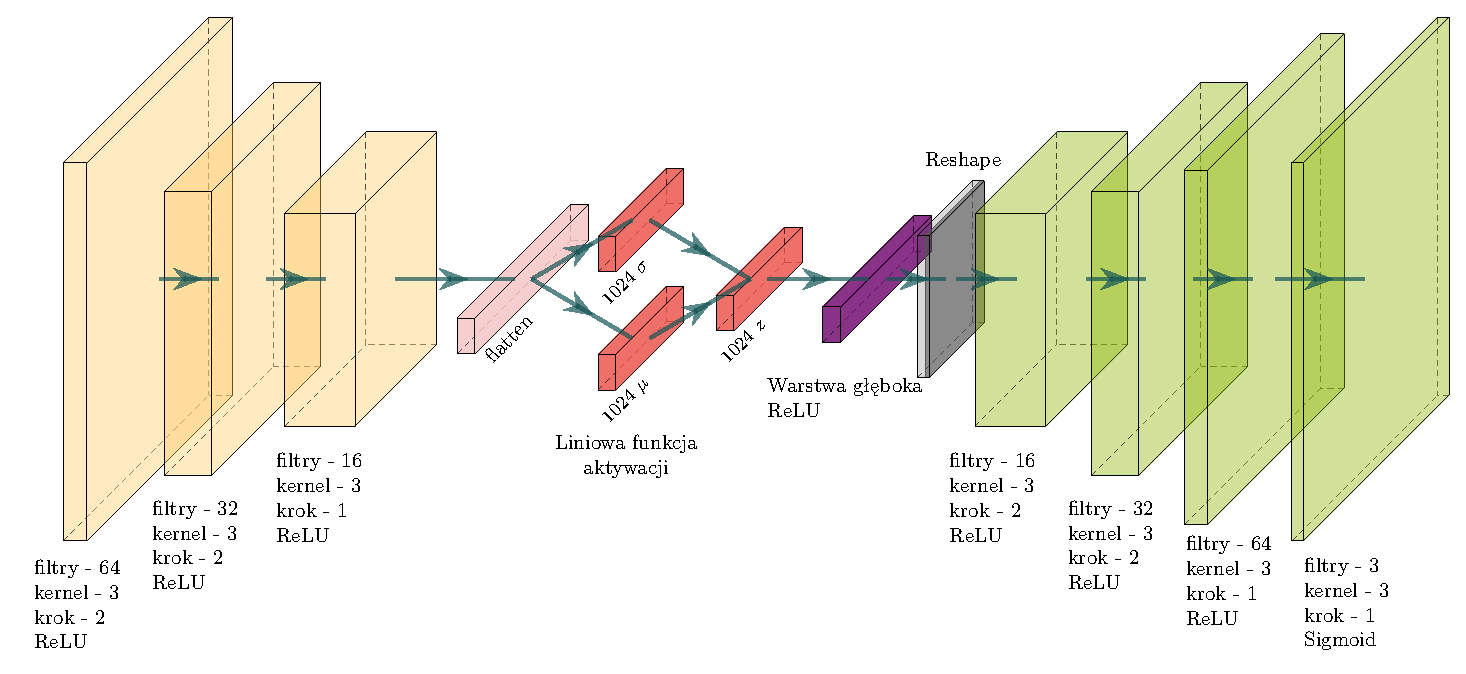
\includegraphics[width=\linewidth]{my_arch.pdf}
	\caption{Architektura modelu konwolucyjnego wariacyjnego autoenkodera}
	\label{fig:convvae}
\end{figure}

Rysunek \ref{fig:vaefacerecon} przedstawia dwa rzędy obrazów, gdzie w rzędzie a są obrazy wchodzące do modelu oraz w b ich rekonstrukcje. Jak można zaobserwować, model skupia się na najważniejszych elementach, takich jak usta, oczy oraz nos. Gorzej zrekonstruowanymi elementami są włosy czy tło. 
\newpage
\begin{figure}[h!]
	\centering
	\begin{tikzpicture}
		\node (face) at (3, 0) {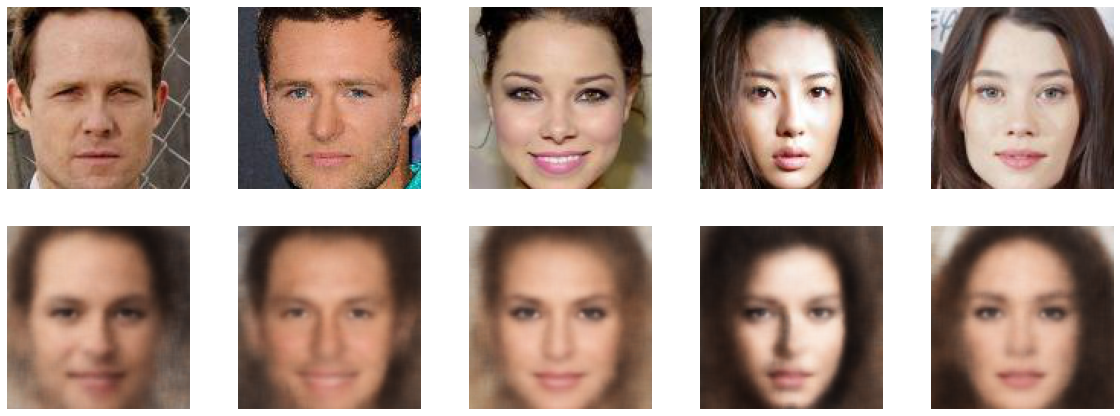
\includegraphics[width=12cm]{facerecon.png}};
		\node (a) at (-3.5, 1.1) {a)};
		\node (b) at (-3.5, -1.1) {b)};
	\end{tikzpicture}
	\caption{Rekonstrukcja twarzy modelem VAE}
	\label{fig:vaefacerecon}
\end{figure}

Aby wygenerować nową twarz, wystarczy wylosować punkt z 1024-wymiarowego rozkładu normalnego, a następnie przekazać go na wejście do dekodera.
\begin{figure}[h!]
	\centering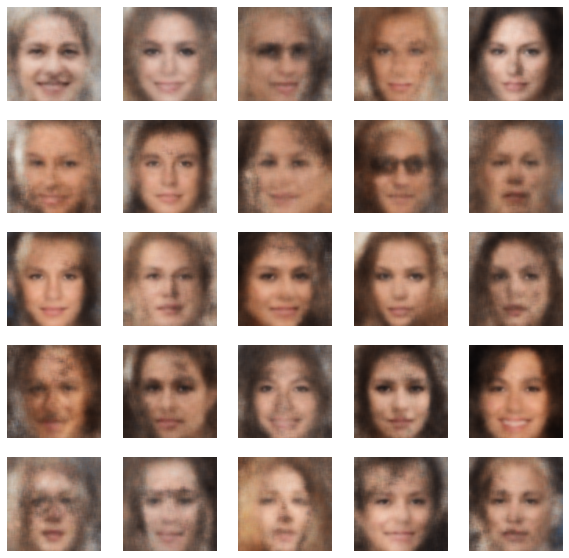
\includegraphics[width=10cm]{generatedfaces.png}
	\caption{Generacja nowych twarzy}
	\label{fig:facegenvae}
\end{figure}

Twarze zaprezentowane na rysunku \ref{fig:facegenvae} są całkowicie nowe. Jak widać na obrazie, model jest w stanie dość dobrze wygenerować podstawowe elementy twarzy jak oczy, nos, usta. W zależności od wylosowanych wartości, twarz może mieć uśmiech, zamknięte usta, różne odcienie koloru skóry lub koloru włosów. Elementy, które nie są obecne na wystarczającej liczbie danych wejściowych, takie jak okulary, nie będą dobrze zrekonstruowane przez model. Wynika to niewystarczającej ilości danych treningowych.


\newpage
\section{Wnioski}
Wariacyjny autoenkoder rozwiązuje problemy generacyjne tradycyjnego modelu. Model VAE implementuje wnioskowanie wariacyjne i dzięki tej metodzie enkoder jest w stanie przybliżyć swoją dystrybucję, aby była jak najbardziej podobna do rozkładu normalnego $\mathcal{N}(0, 1)$. Użycie dywergencji Kullbacka-Leiblera w funkcji straty, zmusza model do nauki wybranego przez nas rozkładu. W ten sposób można wybierać losowo punkty, na podstawie których generowane są nowe dane. Pomimo zmian w sposobie treningu, model dalej jest w stanie być używany do takich samych zastosowań jak tradycyjna architektura, czyli między innymi odszumianie oraz kompresja danych. Budowa modelu jest nietypowa, ponieważ wybierając dystrybucję, trzeba dla każdego parametru charakteryzującego ją stworzyć warstwę, która uczy się tego konkretnego parametru dla każdego wymiaru kodu. Sprawia to problemy implementacji w wybranej technologii, ponieważ warstwy te muszą być rozłączone pomiędzy sobą, ale jednocześnie połączone z poprzednia i następną warstwą, co pokazuje rysunek \ref{fig:vaenetwork} \cite{tikzvae}. 


\chapter{Implementacja}
\section{TensorFlow oraz Keras}
\subsection{Informacje ogóle}
TensorFlow jest jedną z najbardziej popularnych bibliotek implementującą metody uczenia maszynowego. Twórcą projektu jest Google, które udostępniło je jako wolne oprogramowanie \cite{tensorflow2015-whitepaper}. Biblioteka jest dostępna dla wielu języków programowania, jednak najczęściej jest używana w języku Python. Programowanie bezpośrednio w TensorFlow jest dość skomplikowane, a kod jest mało czytelny. Problemy te rozwiązuje Keras, który jest nakładką na bibliotekę. 

Keras również jest darmową i otwartą biblioteką, jednak jest tylko przeznaczona dla języka Python \cite{chollet2015keras}. Implementuje prosty i przejrzysty sposób tworzenia modeli oraz sieci  neuronowych. Poza tradycyjnymi, głębokimi architekturami możliwe jest tworzenie sieci rekurencyjnych oraz konwolucyjnych. Obie biblioteki wspierają rozproszone obliczenia na kartach graficznych. 

W implementacji modeli AE i VAE, użyteczną biblioteką jest NumPy \cite{numpy}. To wolny projekt, ciągle wspierany przez kontrybutorów, umożliwiający operacje na macierzach oraz wektorach. Jako biblioteka napisana w języku C, dokonuje o wiele szybszych operacji w porównaniu do tych, które wykonywane by były w czystym Pythonie. 

Istnieje kilka możliwości implementacji tradycyjnego oraz wariacyjnego autoenkodera przy użyciu sieci gęstych, konwolucyjnych lub nawet rekurencyjnych takich jak LSTM (\textit{long short-term memory}). Każda z nich może nadać się do innych zbiorów danych, jednak wszystkie w kluczowych punktach działają w ten sam sposób. Wejście zostaje skompresowane do odpowiedniej długości kodu, a w przypadku autoenkoderów wariacyjnych do wielowymiarowego rozkładu normalnego. 
\subsection{Implementacja w języku Python}
Potrzebne klasy i pakiety są importowane w listingu \ref{code:imprt}.
\begin{code}[h!]
	\centering
	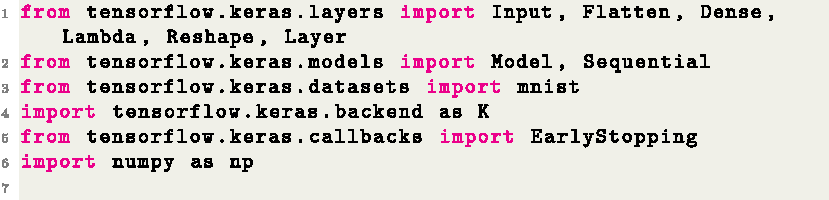
\includegraphics[width=\linewidth]{importy.pdf}
	\caption{Importy klas i funkcji}
	\label{code:imprt}
\end{code}

Następnie wczytany zbiór danych MNIST jest dzielony na część przeznaczone do treningu oraz do testów. Modele AE i VAE nie korzystają z oznaczeń, do jakiej klasy należą poszczególne dane, ponieważ oba modele na swoją warstwę wejściową, jak i wyjściową dostają te same obrazy. Aby nie było problemów z typem danych, najlepiej zamienić wszystkie próbki na macierze, które przechowują dane w formacie float o długości 32 bitów. Następnie dane są skalowane do przedziału [0, 1], dzieląc każdy piksel każdego obrazka przez 255. Dane składają się z obrazów w skali szarości i każdy piksel opisuje liczba z przedziału [0, 255], więc zwykłe dzielenie może zastąpić inne rozwiązania skalowania danych. Zapisano do zmiennych wysokość i szerokość obrazów, aby prościej się do nich odwoływać.
\begin{code}[h!]
	\centering
	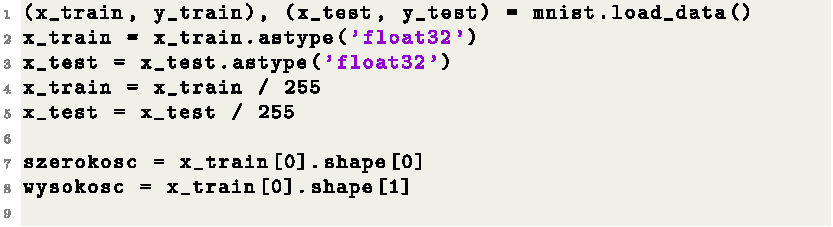
\includegraphics[width=\linewidth]{dane.pdf}
	\caption{Przygotowanie zbioru danych}
	\label{code:dataset}
\end{code}
\subsubsection{Autoenkoder}
 W listingu \ref{code:createae} tworzony jest enkoder z dwiema warstwami ukrytymi, z czego pierwsza posiada 500 neuronów, a druga 120. Obraz jest kompresowany do kodu o długości 2. Architektura dekodera jest odbiciem lustrzanym enkodera. Funkcje aktywacji warstw ukrytych to ReLU \textit{Rectified Linear Unit}, które nie tylko umożliwiają lepszą naukę sieci, ale również sprawiają, że trening zajmuje mniej czasu \cite{relu}. Użyta funkcja liniowa w warstwie kodu nie ogranicza wartości, jakie poszczególne jego elementy mogą przyjąć. Funkcja sigmoidalna na wyjściu spłaszcza wyjście neuronu do przedziału [0, 1], czyli takiego samego, w jakim występują dane.\\

Pierwsza warstwa jest przeznaczona, aby przyjmować dane o wymiarze takim jak obrazy. Następnie warstwa \textit{Flatten} zamienia dwuwymiarowe wejście na jednowymiarowe. Kolejne warstwy łączą się w normalny sposób pomiędzy sobą. Ostatnia warstwa \textit{Reshape} dokonuje odwrotnej operacji co \textit{Flatten}, zamieniając jednowymiarowe wartości na macierz, która ma takie same wymiary co dane wejściowe, co umożliwia porównanie wyniku modelu do wejścia. Do stworzenia całego autoenkodera używa się klasy \textit{Model}, podając pierwszą oraz ostatnią warstwę. W ten sposób wszystkie parametry są trenowane na raz. Stworzenie osobno enkodera nie stanowi problemu, ponieważ posiada on tą samą warstwę wejściową co cały model. Dekoder jest trudniejszy w implementacji, ponieważ należy stworzyć jego własną warstwę wejściową, a następnie połączyć z nią warstwy modelu tak, aby korzystał z wytrenowanych parametrów. 
\begin{code}[h!]
	\centering
	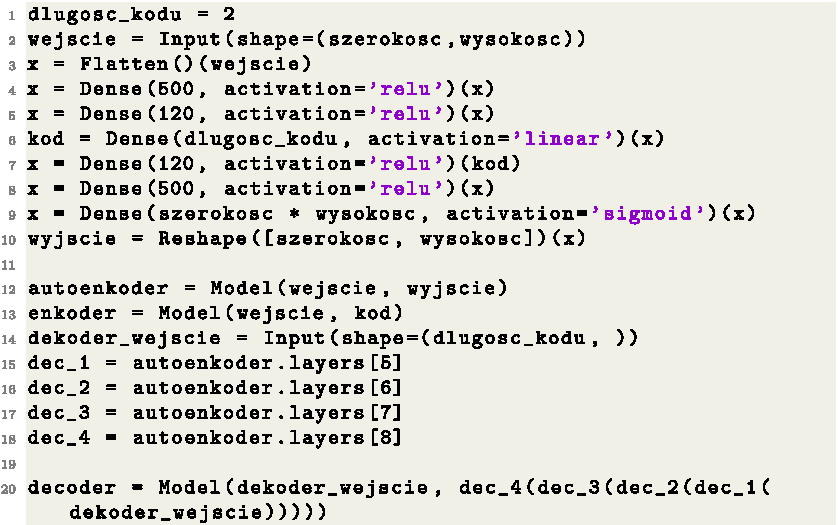
\includegraphics[width=\linewidth]{modelae.pdf}
	\caption{Stworzenie autoenkodera}
	\label{code:createae}
\end{code}

Zanim trening sieci się rozpocznie, trzeba sprecyzować funkcję straty oraz optymalizator. Funkcja użyta w przykładzie \ref{code:trainae} to błąd średniokwadratowy, który jest dobrym wyborem w przypadku porównywania obrazów. Optymalizator to algorytm znajdowania wag parametrów, dla których funkcja straty jest jak najmniejsza, a co za tym idzie model działa jak najlepiej. Wybraną metodą jest algorytm \textit{adam}, który jest pochodną stochastycznego gradientu. Obliczenia okupują mniej pamięci, jest prosty obliczeniowo oraz znajduje optymalne rozwiązanie szybciej niż tradycyjne podejście \cite{adam}. Jednym z jej twórców jest Diedrik Kingma, który również jako pierwszy zaproponował model wariacyjnego autoenkodera. Aby nie przetrenować modelu, dodaje się zbiór walidacyjny, który przejmuje 20\% danych treningowych. Walidacja służy do sprawdzenia na innych danych niż testowe i treningowe, czy model się nie przetrenował. W momencie, kiedy błąd na zbiorze walidacyjnym będzie rosnąć przez 3 epoki zamiast maleć, callback \textit{EarlyStopping} przerwie trening i przywróci wagi do tych, dla których wynik był najlepszy.
\begin{code}[h!]
	\centering
	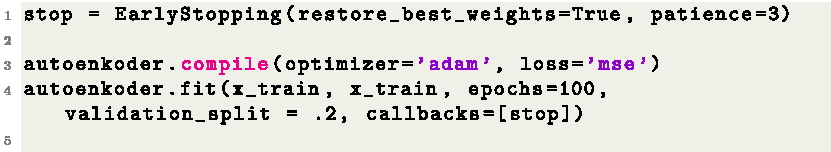
\includegraphics[width=\linewidth]{trainae.pdf}
	\caption{Trening modelu}
	\label{code:trainae}
\end{code}

Po treningu modele są już gotowe go używania. Aby dokonać przy ich pomocy obliczeń, należy wykonać metodę \textit{predict}, do której trzeba podać odpowiednich wymiarów macierz. 
\subsubsection{Wariacyjny autoenkoder}
Przygotowanie zbioru danych dla wariacyjnego autoenkodera nie różni się w żaden sposób od pokazanego w \ref{code:dataset}. 

Implementacja modelu VAE jest bardziej skomplikowana niż AE. Bierze się to z jego budowy, która wymaga rozłączenia jednej warstwy na dwie niezależne, przyłączone do tej samej, co widać na obrazku \ref{fig:vaenetwork} oraz implementacji własnej funkcji straty. Warstwy reprezentujące średnią i odchylenie standardowe są połączone z ostatnią warstwą ukrytą. W listingu \ref{code:createvae} warstwę odchyleń standardowych traktuje się jako ich logarytm, ponieważ jego wartość nie może być ujemna. Kiedy potrzeba użyć zmiennych, wystarczy dokonać na nich operacji \textit{exp}. Funkcja \textit{probka} dokonuje losowania z dystrybucji na nauczonych parametrach, stosując opisaną wcześniej metodę reparametryzacyjną. Zmienna \textit{eps} przechowuje wartości losowane z rozkładu normalnego i ich rozmiar jest równy ilości zmiennych ukrytych i wielkości partii danych (\textit{batch size}). Na etapie tworzenia architektury modelu nie wiadomo o wielkości batch-a, więc używając metody \textit{shape}, można ją dynamicznie zmieniać w zależności od przekazanych parametrów. Dostępna w paczce Keras klasa \textit{Lambda} pozwala wywołać wskazaną funkcję na wartościach neuronów. Warstwa jest łączona z obiema wcześniejszymi warstwami na raz. Implementacja dekodera jest identyczna jak dla tradycyjnego autoenkodera pokazanego w \ref{code:createae}. Funkcja straty modelu VAE nie jest możliwa do automatycznego policzenia, tak jak zostało to pokazane w AE. Zmienna \textit{z$\_$odkodowane} przechowuje obraz odkodowany ze zmiennych ukrytych, który będzie porównywany z tym przekazanym na wejście sieci.

\begin{code}[h!]
	\centering
	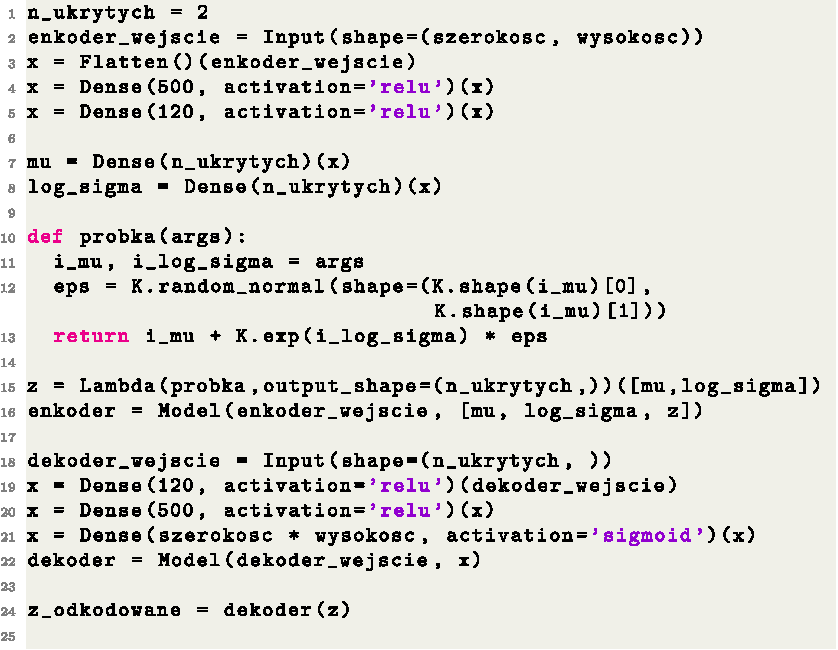
\includegraphics[width=\linewidth]{modelvae.pdf}
	\caption{Stworzenie modelu wariacyjnego autoenkodera}
	\label{code:createvae}
\end{code}

\begin{code}[h!]
	\centering
	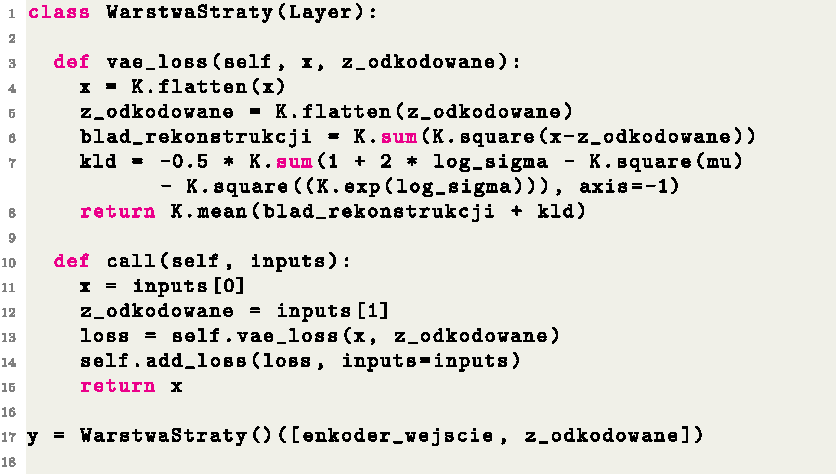
\includegraphics[width=\linewidth]{vaeloss.pdf}
	\caption{Obliczenie warstwy straty VAE}
	\label{code:vaeloss}
\end{code}

\newpage
Aby policzyć wartość funkcji straty, można stworzyć nową warstwę przyłączoną do ostatniej. Jej jedynym zadaniem jest policzenie straty i nie ma ona możliwych do trenowania parametrów. Jej budowa została zaprezentowana na listingu \ref{code:vaeloss}. Pierwsza metoda w klasie oblicza wartość funkcji straty, a druga pozwala na jej policzenie i minimalizację przez model. Aby móc porównać obrazy, muszą być one w takich samych wymiarach, co gwarantuje wywołanie funkcji \textit{flatten} na prawdziwym i odkodowanym obrazie. Błąd rekonstrukcji wybrany w tym przykładzie to błąd średniokwadratowy. Zmienna \textit{kld} przechowuje obliczoną wartość dywergencji Kullbacka-Leiblera z wyprowadzonego wzoru \ref{equ:kld_loss}. Warstwa obliczająca stratę jest połączona z wejściem i wyjściem całego modelu, co umożliwia dostęp do wejścia ze zbioru danych oraz obrazów odkodowanych ze zmiennych ukrytych. 

\begin{code}[h!]
	\centering
	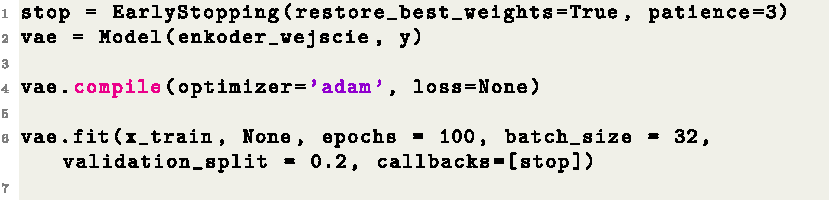
\includegraphics[width=\linewidth]{vaetrain.pdf}
	\caption{Trening modelu}
\end{code}

Posiadając warstwę obliczającą funkcję straty, można stworzyć model. Podczas kompilacji nie należy podawać parametru \textit{loss}, ponieważ został on już dodany w niestandardowej warstwie. Z tego samego powodu w funkcji mającej dokonać treningu modelu nie przekazuje się danych, do których jest porównywany wynik autoenkodera.

\chapter{Podsumowanie}
Autoenkoder tradycyjny oraz wariacyjny są podobnymi modelami uczenia maszynowego. Składają się z dwóch części: enkodera próbującego zakodować zmienne do kodu o określonej długości oraz dekodera rekonstruującego kod do danych wejściowych. Wariacyjny autoenkoder, zamiast generować zmienne bezpośrednio, wybiera je z wielowymiarowego rozkładu normalnego. Jest to sposób na rozwiązanie problemów z generacją nowych danych tradycyjnego modelu. Oba modele posiadają szerokie zastosowanie w kompresji oraz odszumianiu danych i detekcji anomalii. Przewaga wariacyjnego autoenkodera polega na jego umiejętności generacji danych, podobnych do tych, na których on został wytrenowany. 


\listoffigures{}
\addcontentsline{toc}{chapter}{Spis rysunków}

\listofcodes{}
\addcontentsline{toc}{chapter}{Spis Listingów}

%\bibliographystyle{ieeetr}
\printbibliography[title=Bibliografia]
%\bibliography{./cytowania/cytowania}
\addcontentsline{toc}{chapter}{Bibliografia}
\end{document}
